\section{Conception détaillée}

La conception détaillée définit l'architecture logique du système, c'est-à-dire :

\begin{itemize}
    \item répartir le système sur l'architecture matérielle.
    \item gérer les entrées/sorties et les IHM.
    \item élaborer les protocoles de communication.
    \item définir les parallélismes et l'initialisation.
    \item définir le démarrage, l'arrêt, et la destruction du SàE.
\end{itemize}

% Architecture physique
\subsection{Architecture physique}

Le diagramme ci-dessous représente l'architecture physique du programme {\nomLogiciel} et de l'application {\nomApplication} dans leur intégralité. En plus des
classes vues précédemment, ce diagramme présente la gestion de la communication ainsi que les objets frontières nécessaires au bon fonctionnement du système.
Dans ce diagramme, dans un souci de visibilité, nous avons décidé de ne pas détailler les opérations ainsi que les attributs des classes.

\begin{minipage}
    {\linewidth}
    \centering
    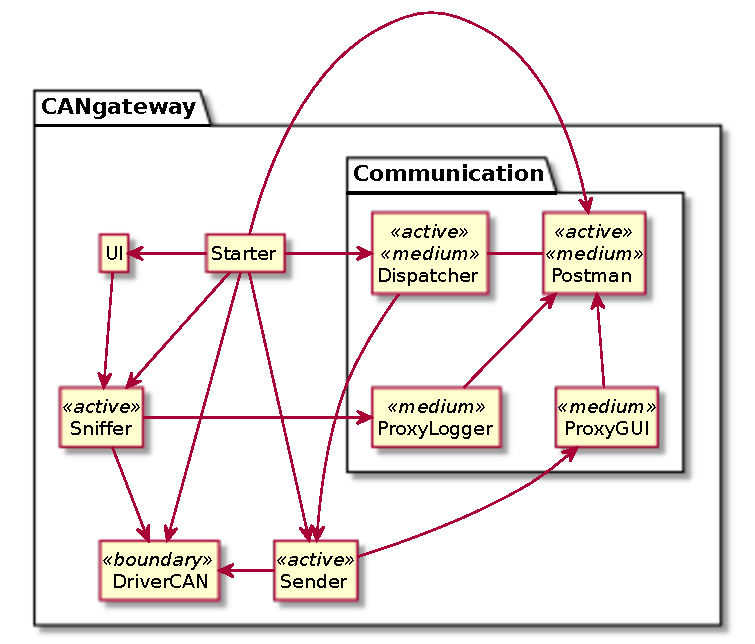
\includegraphics[width=0.8\textwidth]{../schemas/Conception_detaillee/architecture_CANgateway.pdf}
    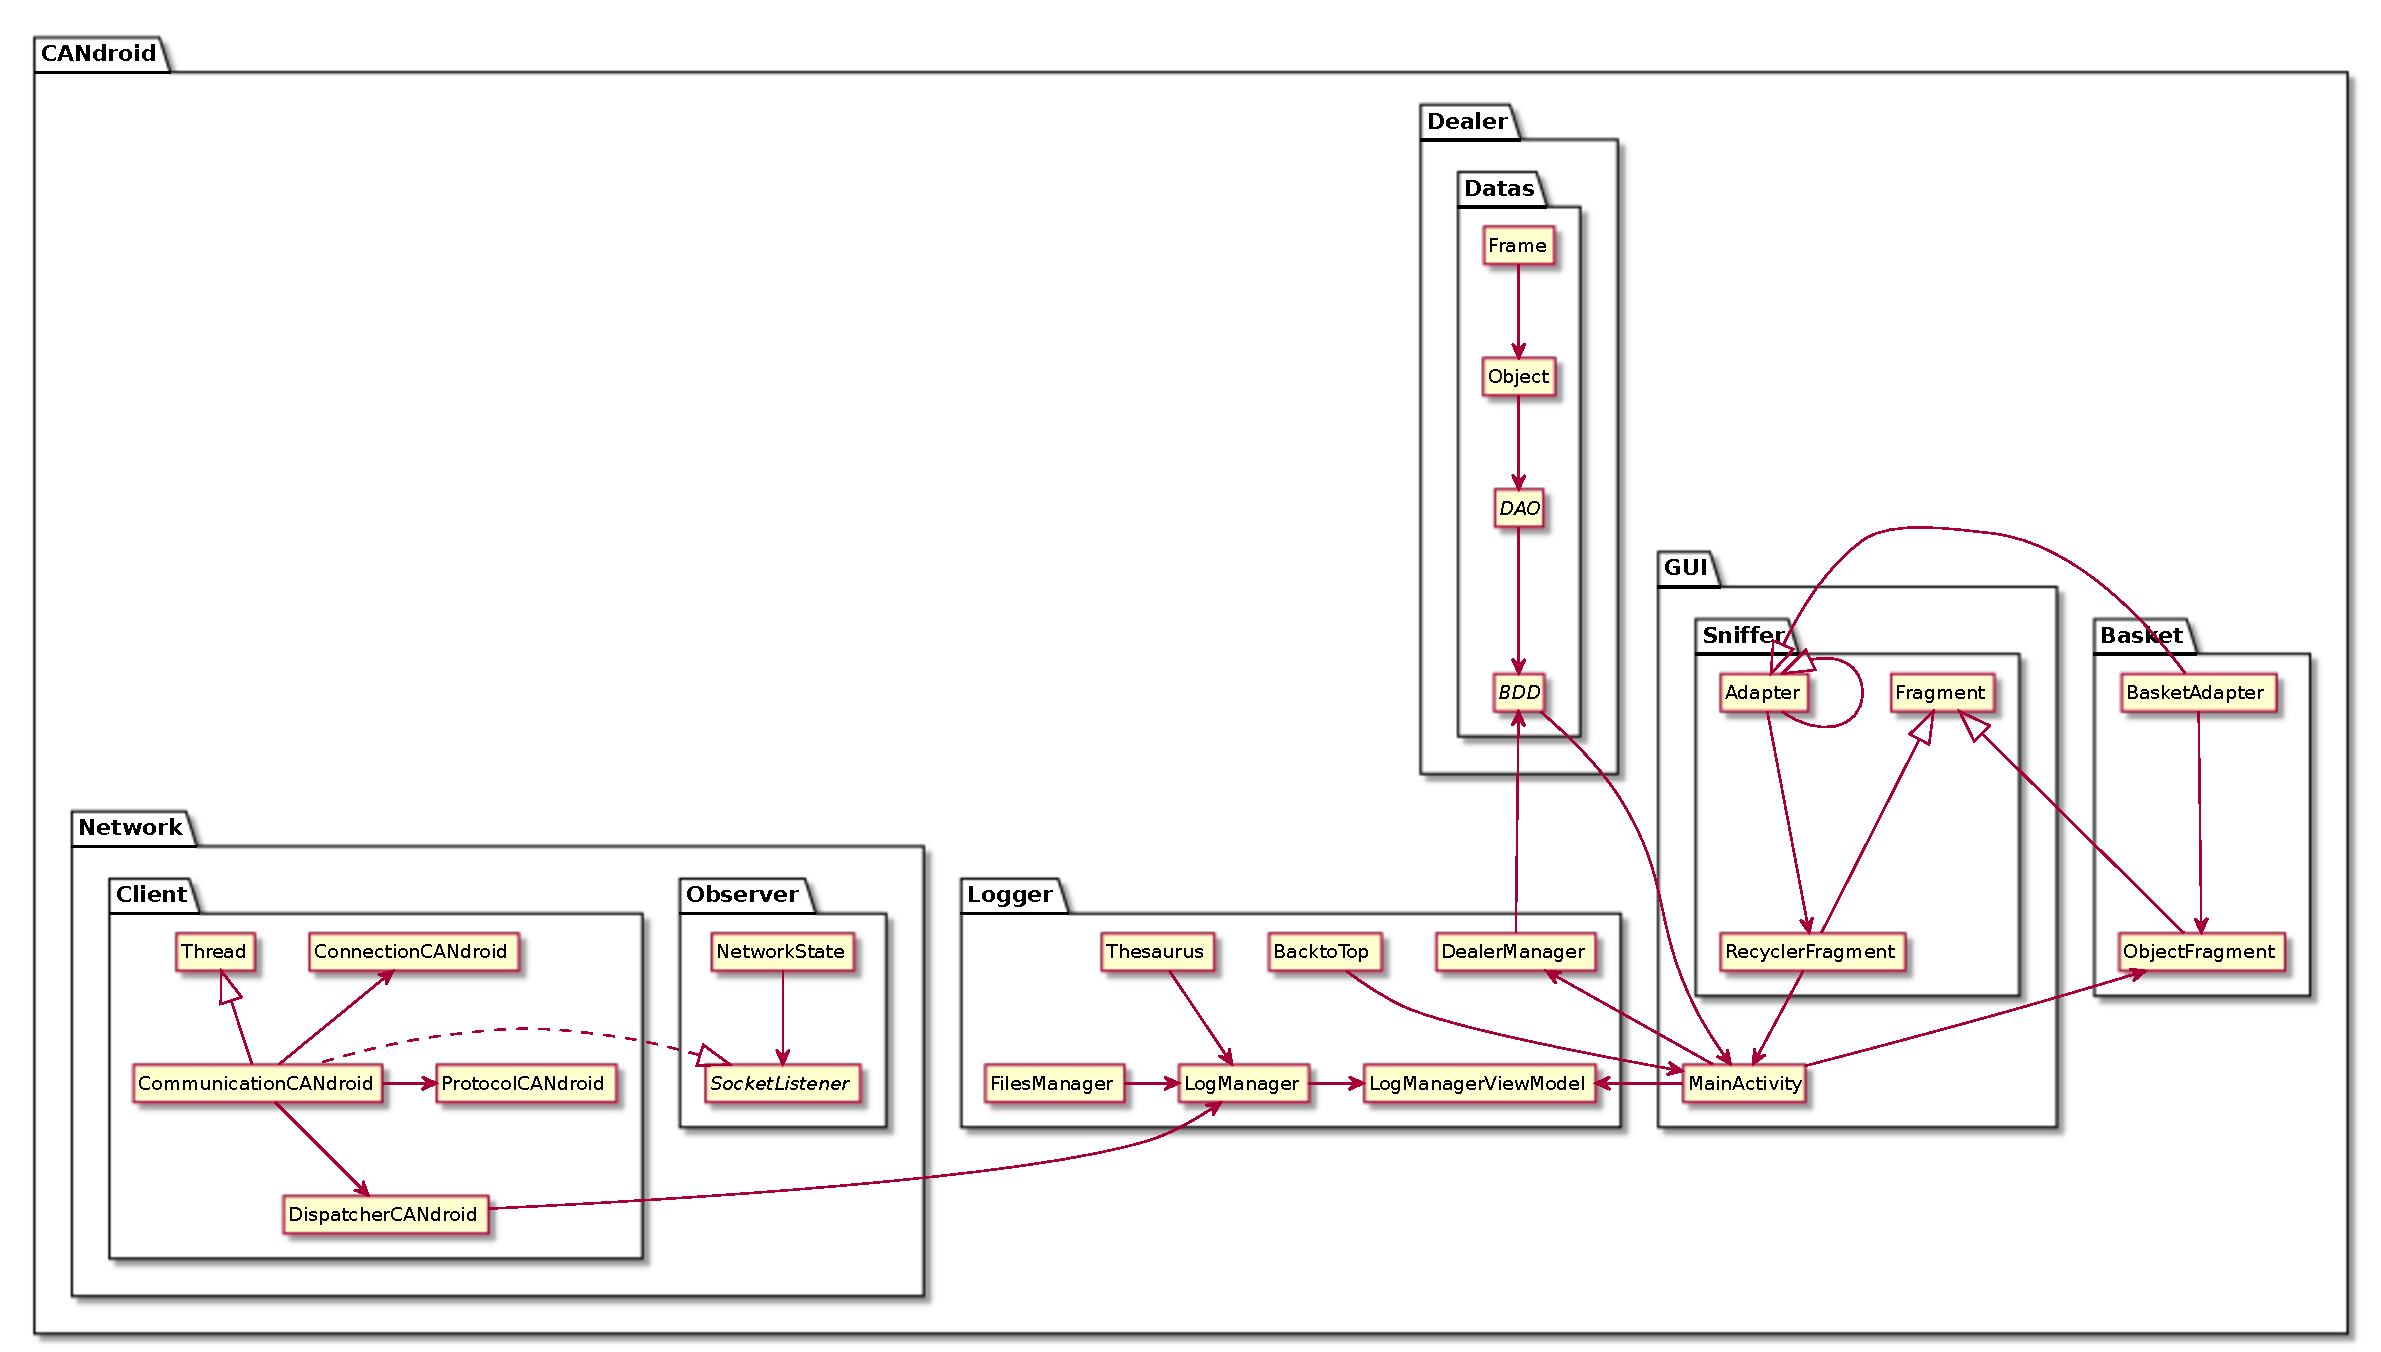
\includegraphics[width=\textwidth]{../schemas/Conception_detaillee/architecture_CANdroid.pdf}
    \captionof{figure}{Architecture physique}
\end{minipage}
\newpage 

% Description des classes
\subsection{Description des classes}

\subsubsection{Description des classes de CANdroid}

Suite à la conception générale, nous avons décidé de diviser certaines classes afin d'améliorer la lisibilité du programme de l'application {\nomApplication}, de faciliter sa réutilisation et son amélioration ultérieure. En effet, certaines classes de la conception générale, telles que Gui, Logger ou encore Basket, sont devenues des packages dans la conception détaillée. Le rôle du package dans la conception détaillée reste identique à celui des classes dans la conception générale. Bien qu'elles aient été divisées, nous fournirons néanmoins une description de chaque classe.

% Diagramme de classe de CANdroid
\paragraph{Diagramme de classes de CANgateway}

\begin{minipage}
    {\linewidth}
    \centering
    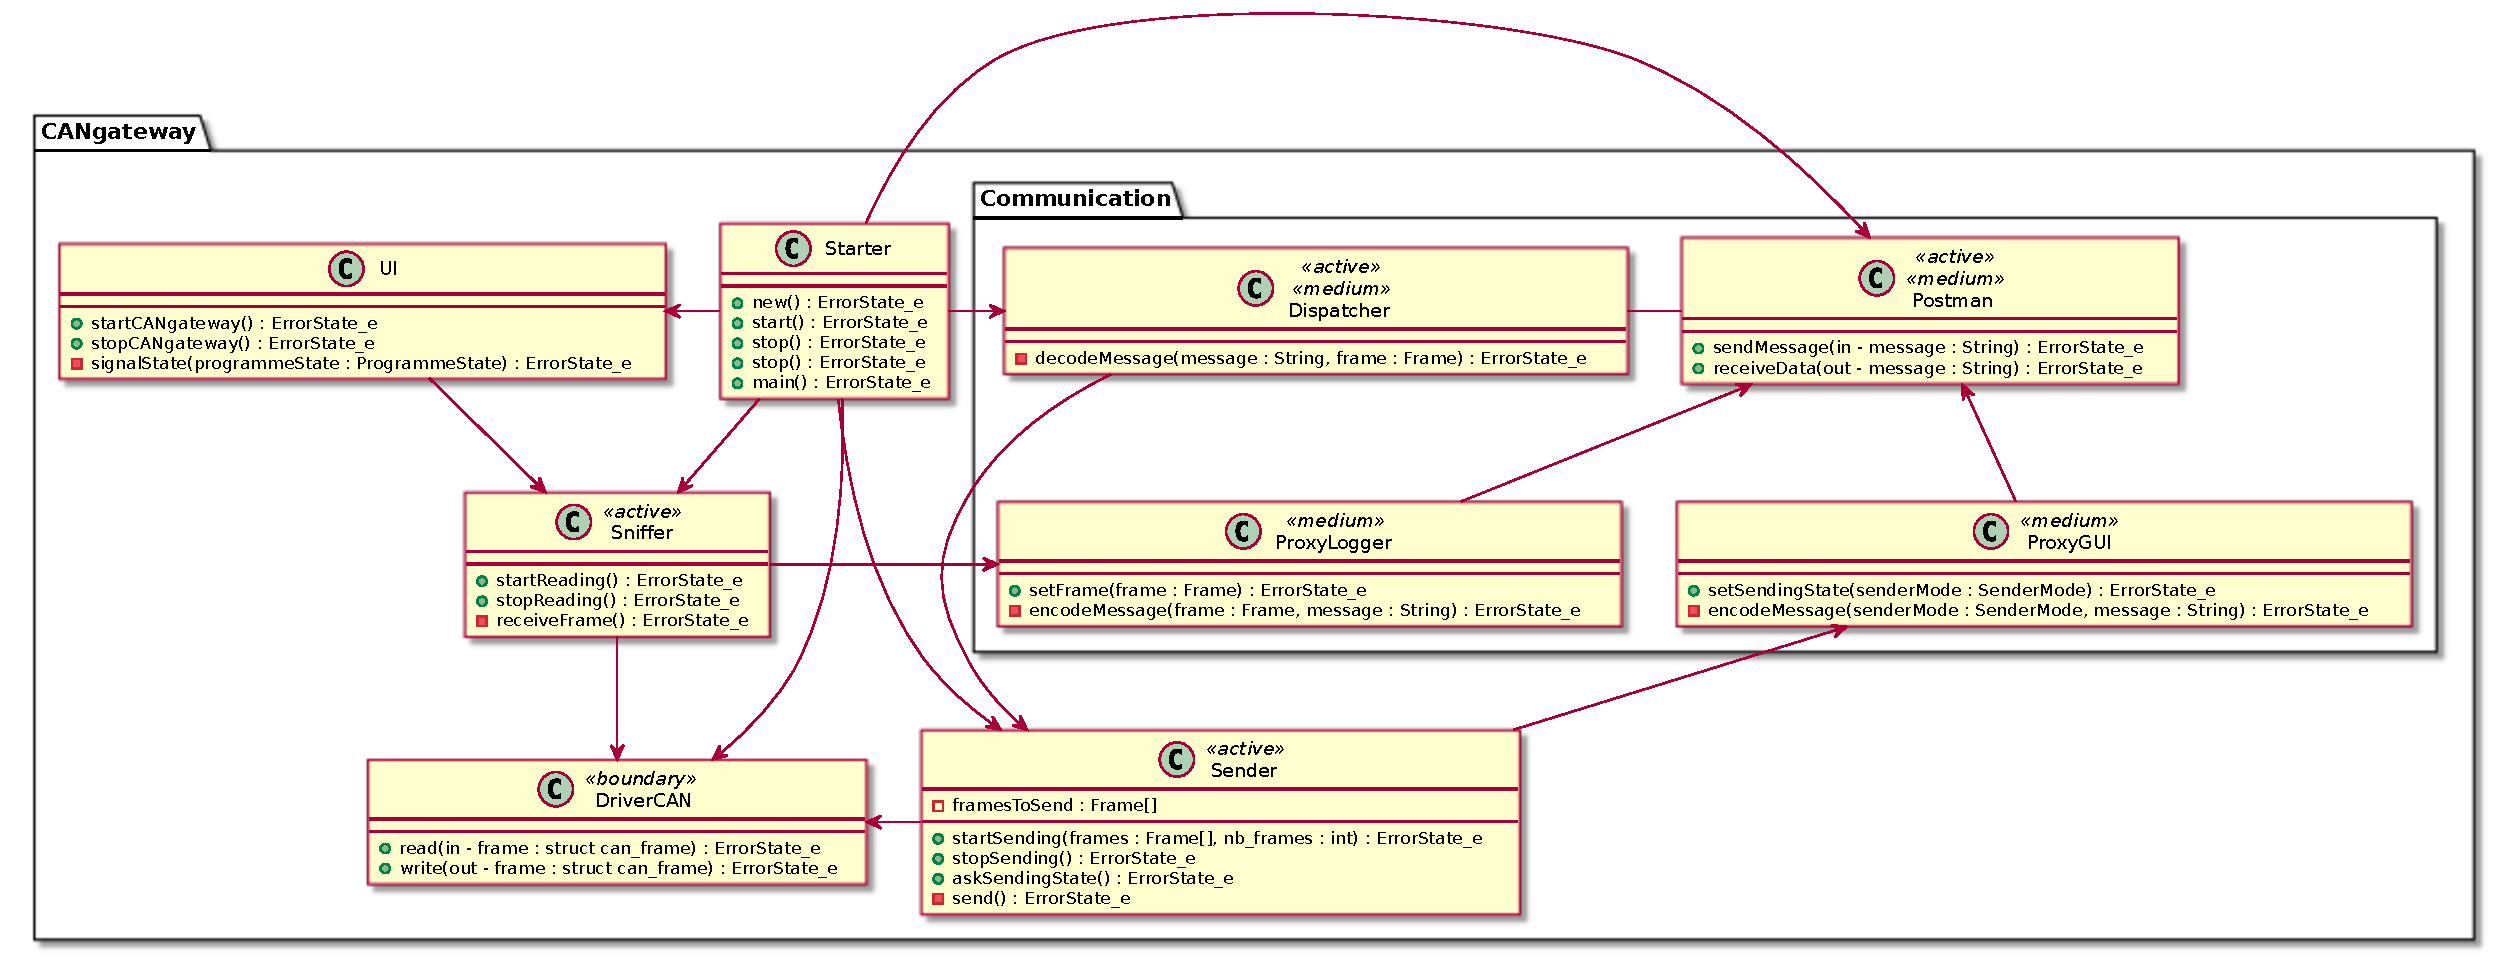
\includegraphics[width=\linewidth]{../schemas/Conception_detaillee/diag_classe_CANgateway.pdf}
    \captionof{figure}{Diagramme de classes de CANgateway}
\end{minipage}

\medspace

Le diagramme de classes de la figure ci-dessus représente l'architecture du programme {\nomLogiciel}. Cette architecture ne respecte pas totalement l'architecture de la conception générale due à l'implémentation d'une gestion d'erreur en C qui change donc les types de retours des fonctions. 
Ces fonctions retournent un état d'erreur de la forme : 
\begin{itemize}
    \item Enumération ErrorState\_e
    \item \'Eléments : 
    \item \begin{itemize}
        \item ERROR\_STATE\_SUCCESS : si tout se passe bien 
        \item ERROR\_STATE\_FAILURE : s'il y a au moins une erreur
        \item ERROR\_STATE\_TIMEOUT : si la cause de l'erreur est un timeout
    \end{itemize}
\end{itemize} 


%% Package Logger %%

% Diagramme de classe de Thesaurus
\paragraph{La classe Thesaurus}

\begin{minipage}
    {\linewidth}
    \centering
    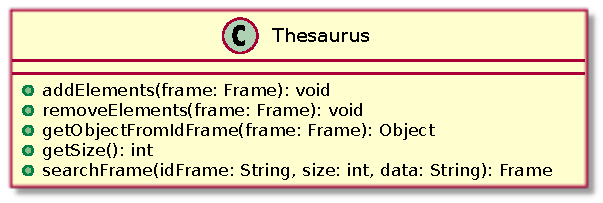
\includegraphics[width=0.80\linewidth]{../schemas/Conception_detaillee/classe_thesaurus.pdf}
    \captionof{figure}{Diagramme de classe de Thesaurus}
\end{minipage}

\subparagraph{Philosophie de conception \newline} 

\medspace

La classe Thesaurus a pour rôle de répertorier sous la forme d'un dictionnaire les trames qui sont envoyées par l'application {\nomApplication}.

\subparagraph{Description structurelle \newline}

\medspace

\textbf{Attributs :}

N.A.

\textbf{Services offerts :}

\begin{itemize}
    \item \textbf{getObjectFromIdFrame(idFrame : String) : Object} --- Opération qui recherche dans le dictionnaire la trame correspondant à l'identifiant "idFrame". Cet identifiant est lié à un objet qui est retourné afin de savoir si un objet contient cette trame.
    \item \textbf{addElements(frame: Frame): void} --- Opération qui permet d'ajouter un élément au dictionnaire.
    \item \textbf{removeElements(frame: Frame): void} --- Opération qui permet de supprimer un élément du dictionnaire. 
    \item \textbf{getObjectFromIdFrame(frame: Frame): Object} --- Opération qui permet de récupérer l'objet à partir d'une trame.
    \item \textbf{getSize(): int} --- Opération qui permet de retourner la taille du dictionnaire. 
    \item \textbf{searchFrame(idFrame: String, size: int, data: String): Frame} --- Opération qui permet de trouver la trame correspondante dans le dictionnaire sans posséder tous les attributs. 
\end{itemize}

% Diagramme de classe de FilesManager
\paragraph{La classe FilesManager}

\begin{minipage}
    {\linewidth}
    \centering
    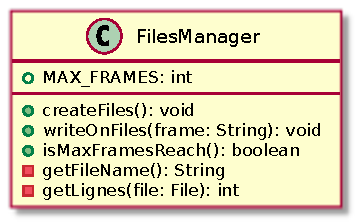
\includegraphics[width=0.80\linewidth]{../schemas/Conception_detaillee/classe_FilesManager.pdf}
    \captionof{figure}{Diagramme de classe de LogManager}
\end{minipage}

\subparagraph{Philosophie de conception \newline} 

\medspace

La classe FilesManager a pour rôle de créer et d'écrire sur un fichier sauvegardé sur le téléphone. 

\subparagraph{Description structurelle \newline}

\medspace

\textbf{Attributs :}

\begin{itemize}
    \item \textbf{MAX\_FRAMES: int} --- Nombre maximal de trames par fichier. 
\end{itemize}

\textbf{Services offerts :}

\begin{itemize}
    \item \textbf{createFiles() : void} --- Opération qui crée le fichier de sauvegarde des trames. 
    \item \textbf{writeOnFiles(frame : String ) : void } --- Opération qui écrit sur le fichier en cours la trame passée en paramètres. 
    \item \textbf{isMaxFramesReach() : bool } --- Opération qui vérifie si le nombre de trames est atteint dans le fichier. 
    \item \textbf{getFileName(): String} --- Opération qui permet de créer le nom du fichier de log.
    \item \textbf{getLignes(file: File): int} --- Opération qui permet de retourner le nombre de lignes présente dans le fichier. 
\end{itemize}

% Diagramme de classe de LogManager
\paragraph{La classe LogManager}

\begin{minipage}
    {\linewidth}
    \centering
    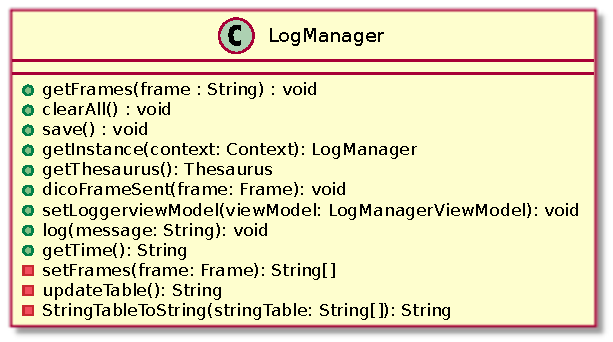
\includegraphics[width=0.80\linewidth]{../schemas/Conception_detaillee/classe_LogManager.pdf}
    \captionof{figure}{Diagramme de classe de LogManager}
\end{minipage}

\subparagraph{Philosophie de conception \newline} 

\medspace

La classe LogManager a pour rôle de traiter les trames reçues depuis la classe DispatcherCANdroid. En effet, lorsque la trame est reçue, elle doit être analysée pour savoir si elle a été envoyée ou non. De plus, elle est mise en forme afin de correspondre à l'affichage. 

\subparagraph{Description structurelle \newline}

\medspace

\textbf{Attributs :}

N.A.

\textbf{Services offerts :}

\begin{itemize}
    \item \textbf{dicoFrameSent(frame : Frame ) : void} --- Opération qui ajoute au dictionnaire la trame envoyée. 
    \item \textbf{setFrame(frame : String ) : String } --- Opération qui met en forme la trame pour l'afficher.
    \item \textbf{getFrames(frame : String ) : void } --- Opération qui récupère les trames reçues. 
    \item \textbf{clearAll() : void } --- Opération qui permet de vider le sniffer en faisant appel à logManagerViewModel. 
    \item \textbf{save() : void } --- Opération qui permet de sauvegarder le fichier en cours.  
    \item \textbf{getInstance(context: Context): LogManager} --- Opération qui permet de retourner une instance de la classe. 
    \item \textbf{getThesaurus(): Thesaurus} --- Opération qui permet de retourner le dictionnaire. 
    \item \textbf{dicoFrameSent(frame: Frame): void} --- Opération qui ajoute au dictionnaire la trame envoyée. 
    \item \textbf{setLoggerviewModel(viewModel: LogManagerViewModel): void} --- Opération qui permet de définir le viewModel. 
    \item \textbf{log(message: String): void} --- Opération qui permet de transmettre le message au viewModel. 
    \item \textbf{getTime(): String} --- Opération qui permet de retourner l'heure. 
    \item \textbf{setFrames(frame: Frame): String[]} --- Opération qui met en forme la trame pour l'afficher. 
    \item \textbf{updateTable(): String} --- Opération qui permet de mettre à jour le tableau comme souhaité pour l'affichage. 
    \item \textbf{StringTableToString(stringTable: String[]): String} --- Opération qui permet de transformer le tableau de String en String.
\end{itemize}

% Diagramme de classe de logMangerViewModel
\paragraph{La classe LogManagerViewModel}

\begin{minipage}
    {\linewidth}
    \centering
    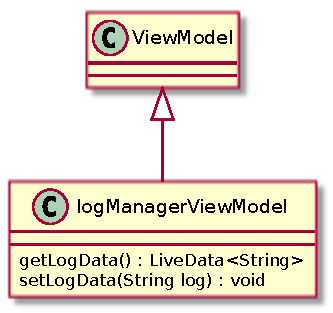
\includegraphics[width=0.80\linewidth]{../schemas/Conception_detaillee/classe_logManagerViewModel.pdf}
    \captionof{figure}{Diagramme de classe de LogManagerViewModel}
\end{minipage}

\subparagraph{Philosophie de conception \newline} 

\medspace

La classe LogManagerViewModel permet de faire le lien entre la vue du sniffer et les sources de données adjacentes. 

\subparagraph{Description structurelle \newline}

\medspace

\textbf{Attributs :}

N.A.

\textbf{Services offerts :}

\begin{itemize}
    \item \textbf{getLogData() : LiveData<String>} --- Opération qui a pour but de stocker des chaînes de caractères représentant les messages de trames. 
    \item \textbf{setLogData(log : String) : void} --- Opération qui permet de mettre à jour l'interface utilisateur en fonction des changements de logData. 
\end{itemize}



%% Package Dealer

% Diagramme de classe de l'interface DAO
\paragraph{L'interface DAO}

\begin{minipage}
    {\linewidth}
    \centering
    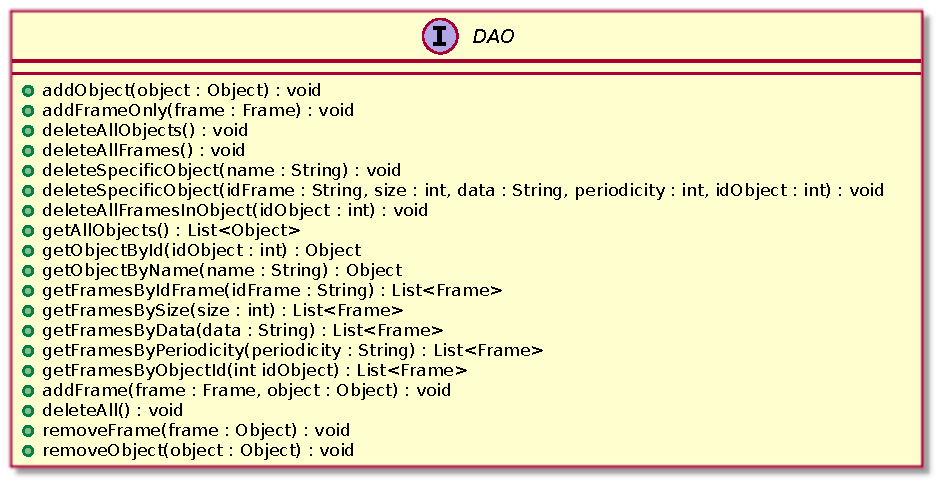
\includegraphics[width=0.80\linewidth]{../schemas/Conception_detaillee/interface_dao.pdf}
    \captionof{figure}{Diagramme de l'interface DAO}
\end{minipage}

\subparagraph{Philosophie de conception \newline} 

\medspace

L'interface DAO définit les différents accès possibles à la base de données.

\subparagraph{Description structurelle \newline}

\medspace

\textbf{Attributs :}

N.A. 


\textbf{Services offerts :}

\begin{itemize}
    \item \textbf{addObject(object : Object) : void } --- Opération qui permet d'ajouter un objet à la base de données.
    \item \textbf{addFrameOnly(frame : Frame) : void } --- Opération qui permet d'ajouter une trame à la base de données.
    \item \textbf{deleteAllObjects() : void } --- Opération qui permet de supprimer tous les objets de la base de données. 
    \item \textbf{deleteAllFrames() : void } --- Opération qui permet de supprimer toutes les trames de la base de données.
    \item \textbf{deleteSpecificObject(name : String) : void } --- Opération qui permet de supprimer un objet précis dans la base de données.
    \item \textbf{deleteSpecificFrame(idFrame : String, size : int, data : String, periodicity : int, idObject : int) : void } --- Opération qui permet de supprimer une trame précise dans la base de données. 
    \item \textbf{deleteAllFramesInObject(idObject : int) : void } --- Opération qui permet de supprimer toutes les trames dans un objet. 
    \item \textbf{getAllObjects() : List<Object> } --- Opération qui permet de sélectionner tous les objets créés. 
    \item \textbf{getObjectById(idObject : int) : Object } --- Opération qui permet de chercher un objet selon son identifiant. 
    \item \textbf{getObjectByName(name : String) : Object } --- Opération qui permet de chercher un objet selon son nom. 
    \item \textbf{getFramesByIdFrame(idFrame : String) : List<Frame> } --- Opération qui permet de chercher une ou plusieurs trames selon leur identifiant de trame.
    \item \textbf{getFramesBySize(size : int) : List<Frame> } --- Opération qui permet de chercher une ou plusieurs trames selon leur taille.
    \item \textbf{getFramesByData(data : String) : List<Frame> } --- Opération qui permet de chercher une ou plusieurs trames selon leur message.
    \item \textbf{getFramesByPeriodicity(periodicity : String) : List<Frame> } --- Opération qui permet de chercher une ou plusieurs trames selon leur périodicité.
    \item \textbf{getFramesByObjectId(int idObject) : List<Frame> } --- Opération qui permet de chercher une ou plusieurs trames selon leur identifant d'objet.
    \item \textbf{addFrame(frame : Frame, object : Object) : void } --- Opération qui permet d'ajouter une trame en fonction d'un objet. Cette opération appelle l'opération qui ajoute la trame à la base de données tout en la liant avec un objet. 
    \item \textbf{deleteAll() : void } --- Opération qui permet de supprimer tous les éléments de la base de données. 
    \item \textbf{removeFrame(frame : Object) : void } --- Opération qui permet de supprimer une trame précisement en ne fournissant en paramètre que la trame à supprimer au lieu des différents paramètres. 
    \item \textbf{removeObject(object : Object) : void } --- Opération qui permet de supprimer un objet précisement en ne fournissant en paramètre que l'objet à supprimer au lieu des différents paramètres.  
\end{itemize}



% Diagramme de classe de BDD
\paragraph{La classe BDD}


\begin{minipage}
    {\linewidth}
    \centering
    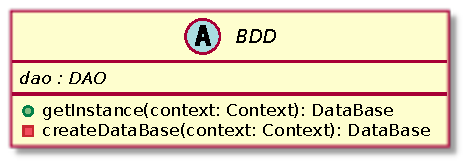
\includegraphics[width=0.30\linewidth]{../schemas/Conception_detaillee/classe_bdd.pdf}
    \captionof{figure}{Diagramme de classe de BDD}
\end{minipage}
\subparagraph{Philosophie de conception \newline} 

\medspace

La classe BDD a pour rôle d'instancier l'interface DAO.  

\subparagraph{Description structurelle \newline}

\medspace

\textbf{Attributs :}

\begin{itemize}
    \item \textbf{dao : DAO} --- Opération qui permet d'instancier l'interface DAO. 
    \item \textbf{getInstance(context: Context): DataBase} --- Opération qui de créer une instance de la base de données.
    \item \textbf{createDataBase(context: Context): DataBase} --- Opération qui de créer la base de données. 
\end{itemize}

\textbf{Services offerts :}

N.A.



% Diagramme de classe de Object
\paragraph{La classe Object}

\begin{minipage}
    {\linewidth}
    \centering
    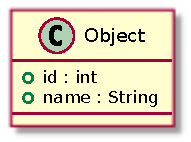
\includegraphics[width=0.80\linewidth]{../schemas/Conception_detaillee/classe_object.pdf}
    \captionof{figure}{Diagramme de classe de Object}
\end{minipage}

\subparagraph{Philosophie de conception \newline} 

\medspace

La classe Object définit les attributs des objets. 

\subparagraph{Description structurelle \newline}

\medspace

\textbf{Attributs :}

\begin{itemize}
    \item \textbf{id : int} --- Identifiant unique et interne à l'application de l'objet afin de l'identifier. 
    \item \textbf{name : String } --- Nom de l'objet. 
\end{itemize}


\textbf{Services offerts :}

N.A.

% Diagramme de classe de Frame
\paragraph{La classe Frame}

\begin{minipage}
    {\linewidth}
    \centering
    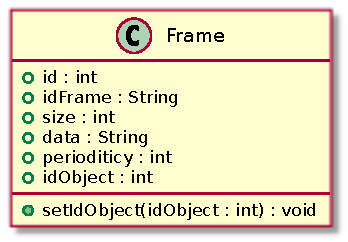
\includegraphics[width=0.80\linewidth]{../schemas/Conception_detaillee/classe_frame.pdf}
    \captionof{figure}{Diagramme de classe de Frame}
\end{minipage}

\subparagraph{Philosophie de conception \newline} 

\medspace

La classe Frame définit les attributs des trames. 

\subparagraph{Description structurelle \newline}

\medspace

\textbf{Attributs :}

\begin{itemize}
    \item \textbf{id : int} --- Identifiant unique et interne à l'application de la trame afin de l'identifier. 
    \item \textbf{idFrame : String} --- Identifant de la trame. 
    \item \textbf{size : int} --- Taille de la trame.
    \item \textbf{data : String} --- Message de la trame. 
    \item \textbf{periodicity : int} --- Périodicité de la trame, la valeur est à 0 lorsque la trame est ponctuelle. 
    \item \textbf{idObject : int} --- Identifiant permettant de lier un objet à la trame. 
\end{itemize}


\textbf{Services offerts :}

\begin{itemize}
    \item \textbf{setIdObject(idObject : int) : void} --- Opération qui permet de définir l'id de l'object (idObject) avec l'objet associé. Cela permet de créer une relation entre les trames et les objets.  
\end{itemize}

% Diagramme de classe de Dealer
%\paragraph{La classe DealerManager}


\begin{minipage}
    {\linewidth}
    \centering
    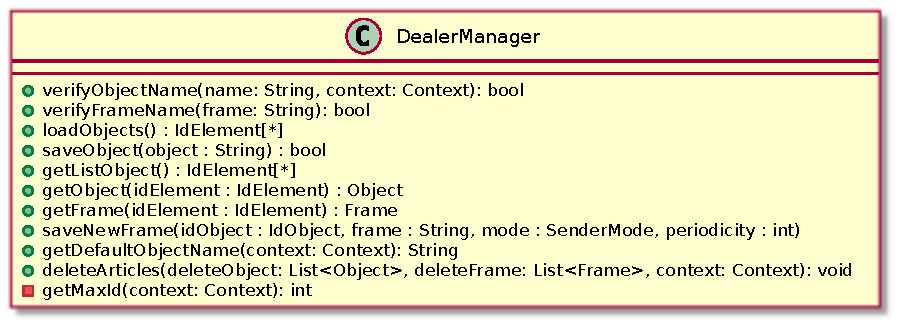
\includegraphics[width=0.80\linewidth]{../schemas/Conception_detaillee/classe_dealer.pdf}
    \captionof{figure}{Diagramme de classe de DealerManager}
\end{minipage}
\subparagraph{Philosophie de conception \newline} 

\medspace

La classe DealerManager permet d'enregistrer les objets et trames enregistrés sur l'application CANdroid. Les opérations étant déjà détaillées dans la conception générale, nous nous contenterons de les lister.
\subparagraph{Description structurelle \newline}

\medspace

\textbf{Attributs :}

N.A.

\textbf{Services offerts :}

\begin{itemize}
    \item \textbf{verifyObjectName(name: String, context: Context): bool}  
    \item \textbf{verifyFrameName(frame: String): bool}
    \item \textbf{loadObjects() : IdElement[*]}  
    \item \textbf{saveObject(object : String) : bool}  
    \item \textbf{getListObject() : IdElement[*]}  
    \item \textbf{getObject(idElement : IdElement) : Object}  
    \item \textbf{getFrame(idElement : IdElement) : Frame}  
    \item \textbf{saveNewFrame(idObject : IdObject, frame : String, mode : SenderMode, periodicity : int)}  
    \item \textbf{getDefaultObjectName(context: Context): String}
    \item \textbf{deleteArticles(deleteObject: List<Object>, deleteFrame: List<Frame>, context: Context): void} 
    \item \textbf{getMaxId(context: Context): int}
\end{itemize}




%% Package Network

% Diagramme de classe de ProtocolCANdroid
\paragraph{La classe ProtocolCANdroid}


\begin{minipage}
    {\linewidth}
    \centering
    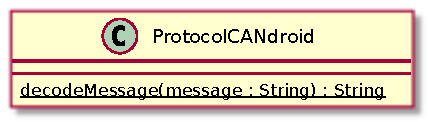
\includegraphics[width=0.50\linewidth]{../schemas/Conception_detaillee/classe_protocolCANdroid.pdf}
    \captionof{figure}{Diagramme de classe de ProtocolCANdroid}
\end{minipage}
\subparagraph{Philosophie de conception \newline} 

\medspace

La classe ProtocolCANdroid a pour rôle de décoder le message reçu par le programme {\nomLogiciel}. 

\subparagraph{Description structurelle \newline}

\medspace

\textbf{Attributs :}

N.A.

\textbf{Services offerts :}

\begin{itemize}
    \item \textbf{decodeMessage(message : String) : String} --- Opération qui permet le décodage du message reçu. L'application {\nomApplication} reçoit \textasciitilde{}frame\#id\$size@message, le décodage permet de retourner \#id\$size@message au dispatcher. 
\end{itemize}



% Diagramme de classe de CommunicationCANdroid
\paragraph{La classe CommunicationCANdroid}

\begin{minipage}
    {\linewidth}
    \centering
    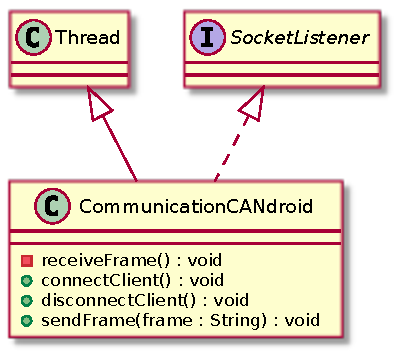
\includegraphics[width=0.5\linewidth]{../schemas/Conception_detaillee/classe_communicationCANdroid.pdf}
    \captionof{figure}{Diagramme de classe de CommunicationCANdroid}
\end{minipage}

\subparagraph{Philosophie de conception \newline} 

\medspace

La classe CommunicationCANdroid a pour rôle d'utiliser les opérations de connexion afin de faire la liaison entre le métier et le logiciel. 

\subparagraph{Description structurelle \newline}

\medspace

\textbf{Attributs :}

N.A.

\textbf{Services offerts :}

\begin{itemize}
    \item \textbf{receiveFrame() : void} --- Opération qui permet de recevoir des trames. 
    \item \textbf{connectClient() : void } --- Opération qui permet de se connecter au programme {\nomLogiciel}. 
    \item \textbf{disconnectClient() : void } --- Opération qui permet de se déconnecter au programme {\nomLogiciel}. 
    \item \textbf{sendFrame(frame : String) : void} --- Opération qui permet d'envoyer les trames au programme {\nomLogiciel}.
\end{itemize}

% Diagramme de classe de ConnectionCANdroid
\paragraph{La classe ConnectionCANdroid}

\begin{minipage}
    {\linewidth}
    \centering
    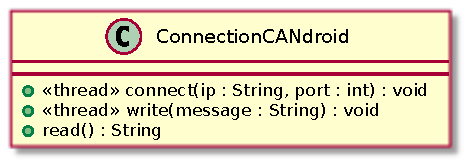
\includegraphics[width=0.5\linewidth]{../schemas/Conception_detaillee/classe_connectionCANdroid.pdf}
    \captionof{figure}{Diagramme de classe de ConnectionCANdroid}
\end{minipage}

\subparagraph{Philosophie de conception \newline} 

\medspace

La classe ConnectionCANdroid a pour rôle de se connecter au programme {\nomLogiciel}, d'envoyer des données et d'en lire. 

\subparagraph{Description structurelle \newline}

\medspace

\textbf{Attributs :}

N.A.

\textbf{Services offerts :}

\begin{itemize}
    \item \textbf{connect(ip : String, port : int) : void} --- Opération qui permet de se connecter au port et à l'IP donnés en paramètres. 
    \item \textbf{write(message : String) : void } --- Opération qui permet d'écrire sur le socket.  
    \item \textbf{read() : String } --- Opération qui permet de lire le socket.
\end{itemize}

% Diagramme d'interface de SocketListener
\paragraph{L'interface SocketListener}


\begin{minipage}
    {\linewidth}
    \centering
    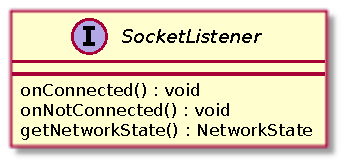
\includegraphics[width=0.30\linewidth]{../schemas/Conception_detaillee/interface_SocketListener.pdf}
    \captionof{figure}{Diagramme de l'interface SocketListener}
\end{minipage}
\subparagraph{Philosophie de conception \newline} 

\medspace

L'interface SocketListener a pour rôle de retourner l'état de la connexion. 

\subparagraph{Description structurelle \newline}

\medspace

\textbf{Attributs :}

N.A.

\textbf{Services offerts :}

\begin{itemize}
    \item \textbf{onConnected() : void} --- Opération qui retourne l'état connecté. 
    \item \textbf{onNotConnected() : void } --- Opération qui retourne l'état non connecté.
    \item \textbf{getNetworkState() : NetworkState } --- Opération qui permet de retourner l'état de la connexion à l'ensemble de l'application. 
\end{itemize}



% Diagramme d'énumeration de NetworkState
\paragraph{L'énumération NetworkState}

\begin{minipage}
    {\linewidth}
    \centering
    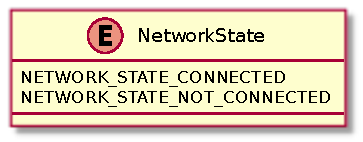
\includegraphics[width=0.5\linewidth]{../schemas/Conception_detaillee/enum_NetworkState.pdf}
    \captionof{figure}{Diagramme de l'énumération NetworkState}
\end{minipage}

\subparagraph{Philosophie de conception \newline} 

\medspace

L'énumération NetworkState a été définie précédemment, ici, les énumérations seront uniquement listées. 

\subparagraph{Description structurelle \newline}

\medspace

\textbf{Attributs :}

N.A.

\textbf{Services offerts :}

\begin{itemize}
    \item NETWORK\_STATE\_CONNECTED
    \item NETWORK\_STATE\_NOT\_CONNECTED
\end{itemize}

% Diagramme de classe de Dispatcher
\paragraph{La classe Dispatcher}


\begin{minipage}
    {\linewidth}
    \centering
    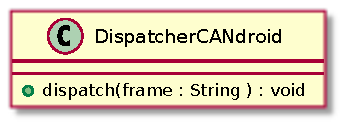
\includegraphics[width=0.50\linewidth]{../schemas/Conception_detaillee/classe_dispatcher_candroid.pdf}
    \captionof{figure}{Diagramme de classe de DispatcherCANdroid}
\end{minipage}
\subparagraph{Philosophie de conception \newline} 

\medspace


La classe DispatcherCANdroid a pour objectif de faciliter la communication. Elle joue le rôle d'intermédiaire entre la classe CommunicationCANdroid et la classe LogManager. Elle permet une communication centralisée et efficace dans l'application {\nomApplication}. 

\subparagraph{Description structurelle \newline}


\medspace

\textbf{Attributs :}

N.A.

\textbf{Services offerts :}

\begin{itemize}
    \item \textbf{dispatch(frame : String) : void} --- Opération qui permet l'envoi de la trame vers logManager pour ensuite l'afficher. 
\end{itemize}


%% Package Sender

% Diagramme de classe de sendFrames
\paragraph{La classe SendFrames}

\begin{minipage}
    {\linewidth}
    \centering
    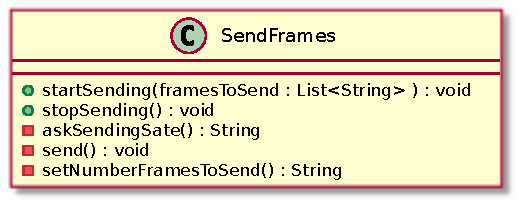
\includegraphics[width=\linewidth]{../schemas/Conception_detaillee/diag_class_sender_client.pdf}
    \captionof{figure}{Diagramme de classe de SendFrames}
\end{minipage}

\subparagraph{Philosophie de conception \newline} 

\medspace

La classe SendFrames a pour rôle d'envoyer les trames au programme {\nomLogiciel}.  

\subparagraph{Description structurelle \newline}

\medspace

\textbf{Attributs :}

N.A.

\textbf{Services offerts :}

\begin{itemize}
    \item \textbf{startSending(framesToSend : List<String>) : void} --- Opération qui permet de commencer à envoyer des trames. 
    \item \textbf{stopSending() : void } --- Opération qui permet d'arrêter l'envoi des trames. 
    \item \textbf{askSendingState() : String } --- Opération qui permet l'envoi de la demande d'état afin de savoir si les trames sont en cours d'envoi ou non. 
    \item \textbf{send() : void} --- Opération qui envoie les différentes informations à envoyer ainsi que les trames. 
    \item \textbf{setNumberFramesToSend() : String } --- Opération qui permet de connaitre le nombre de trames à envoyer et retourne le nombre sous la forme "nb=X" où X est le nombre de trames à envoyer. 
\end{itemize}

%% Package Basket 

% Diagramme de classe de basket
\paragraph{La classe ObjectFragment}

\begin{minipage}
    {\linewidth}
    \centering
    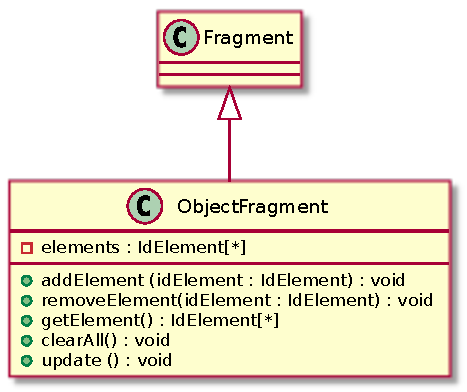
\includegraphics[width=0.80\linewidth]{../schemas/Conception_detaillee/classe_basket.pdf}
    \captionof{figure}{Diagramme de classe de ObjectFragment}
\end{minipage}

\subparagraph{Philosophie de conception \newline} 

\medspace

La classe ObjectFragment est la classe gère le fragment des objets. Elle a aussi pour objectif d'effectuer les  ajouts et soustractions d'éléments. Les opérations étant déjà détaillées dans la conception générale, elles seront uniquement listées.

\subparagraph{Description structurelle \newline}

\medspace

\textbf{Attributs :}

N.A.

\textbf{Services offerts :}

\begin{itemize}
    \item \textbf{elements : IdElement[*]} 
    \item \textbf{addElement (idElement : IdElement)} 
    \item \textbf{removeElement(idElement : IdElement)} 
    \item \textbf{getElements() : IdElement[*]} 
    \item \textbf{clearAll()} 
    \item \textbf{update () : void}


\end{itemize}


\paragraph{La classe BasketAdapter}

\begin{minipage}
    {\linewidth}
    \centering
    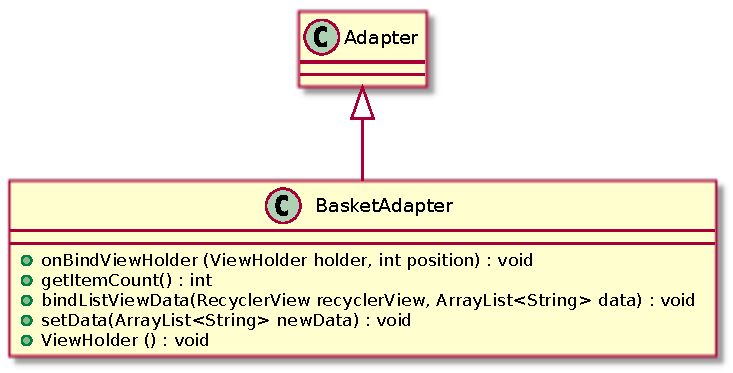
\includegraphics[width=0.80\linewidth]{../schemas/Conception_detaillee/classe_basketAdapter.pdf}
    \captionof{figure}{Diagramme de classe de BasketAdapter}
\end{minipage}

\subparagraph{Philosophie de conception \newline} 

\medspace

La classe BasketAdapter est la classe d'adapter du listView qui gère les items des objets. Elle permet de mettre en forme chaque éléments individuellement et de mettre en forme l'assemblage.

\subparagraph{Description structurelle \newline}

\medspace

\textbf{Attributs :}

N.A.

\textbf{Services offerts :}

\begin{itemize}
    \item \textbf{onBindViewHolder (ViewHolder holder, int position) : void} --- Opération qui permet le binding du ViewHolder. 
    \item \textbf{getItemCount() : int} --- Opération qui permet de retourner le nombre d'items à répartir dans la liste. 
    \item \textbf{bindListViewData(RecyclerView recyclerView, ArrayList<String> data) : void} --- Opération qui permet le binding du listView.
    \item \textbf{setData(ArrayList<String> newData) : void} --- Opération qui permet la mise à jour de la liste.
    \item \textbf{ViewHolder () : void} --- Classe qui permet la création du ViewHolder pour positionner chaque élément individuellement.


\end{itemize}


%% Package GUI

% Diagramme de classe de mainActivity
\paragraph{La classe MainActivity}

\begin{minipage}
    {\linewidth}
    \centering
    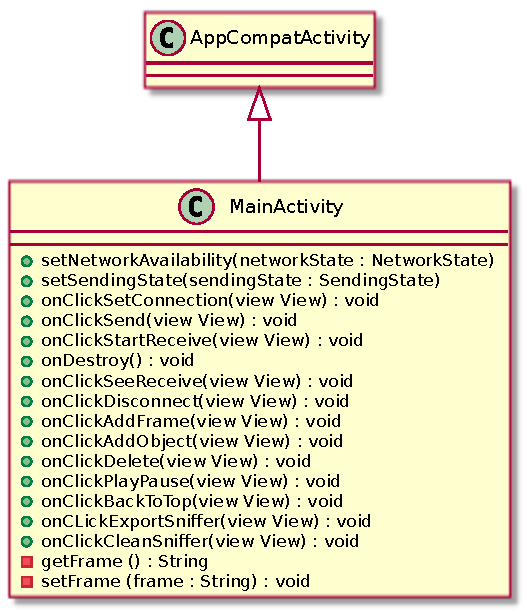
\includegraphics[width=0.60\linewidth]{../schemas/Conception_detaillee/classe_mainActivity.pdf}
    \captionof{figure}{Diagramme de classe de MainActivity}
\end{minipage}

\subparagraph{Philosophie de conception \newline} 

\medspace

La classe MainActivity permet de gérer les interfaces utilisateur de l'application {\nomApplication}. Elle est la classe centrale de l'IHM. 

\subparagraph{Description structurelle \newline}

\medspace

\textbf{Attributs :}

N.A.

\textbf{Services offerts :}

\begin{itemize}
    \item \textbf{setNetworkAvailability(networkState : NetworkState)}  --- Opération qui est appelée lorsqu'on clique sur le bouton de connexion.
    \item \textbf{setSendingState(sendingState : SendingState)}  --- Opération qui permet de mettre à jour l'état d'envoi.
    \item \textbf{onClickSetConnection(view View) : void}  --- Opération qui est appelée lorsqu'on clique sur le bouton de connexion.
    \item \textbf{onClickSend(view View) : void}  --- Opération qui est appelée lorsqu'on clique sur le bouton d'envoi.
    \item \textbf{onClickStartReceive(view View) : void}  --- Opération qui est appelée lorsqu'on clique sur le bouton de réception.
    \item \textbf{onDestroy() : void}  --- Opération qui est appelée lors de la fermeture de l'activité principale. Elle permet la déconnexion. 
    \item \textbf{onClickSeeReceive(view View) : void}  --- Opération qui est appelée lorsqu'on clique sur le bouton d'affichage de la réception.
    \item \textbf{onClickDisconnect(view View) : void}  --- Opération qui est appelée lorsqu'on clique sur le bouton de déconnexion.
    \item \textbf{onClickAddFrame(view View) : void}  --- Opération qui est appelée lors de l'ajout d'une trame dans un objet, par un clique sur le bouton [ajouterTrame].
    \item \textbf{onClickAddObject(view View) : void}  --- Opération qui est appelée lors de l'ajout d'un objet, par un clique sur le bouton [ajouterObjet].
    \item \textbf{onClickDelete(view View) : void}  --- Opération qui est appelée lors de la suppression d'un ou plusieurs éléments. 
    \item \textbf{onClickPlayPause(view View) : void}  --- Opération qui est appelée lors de la mise en pause/play du sniffer. 
    \item \textbf{onClickBackToTop(view View) : void}  --- Opération qui est appelée lorsque Utilisateur souhaite revenir en haut du sniffer.
    \item \textbf{onCLickExportSniffer(view View) : void}  --- Opération qui est appelée lors de l'export du sniffer. 
    \item \textbf{onClickCleanSniffer(view View) : void}  --- Opération qui est appelée lors d'un clique sur le bouton [viderSniffer], c'est à dire, de manière à vider le sniffer des trames actuelles.
    \item \textbf{getFrame () : String}  --- Opération qui est appelée lorsqu'on souhaite récupérer la dernière trame reçue.
    \item \textbf{setFrame (frame : String) : void}  --- Opération qui permet de mettre à jour la dernière trame reçue. 
   
\end{itemize}



% Diagramme de classe de Objects
\paragraph{La classe ObjectAdapter}

La classe ObjectAdapter est une classe du package Objects dont nous détaillerons le rôle pour une meilleure compréhension. 

\begin{minipage}
    {\linewidth}
    \centering
    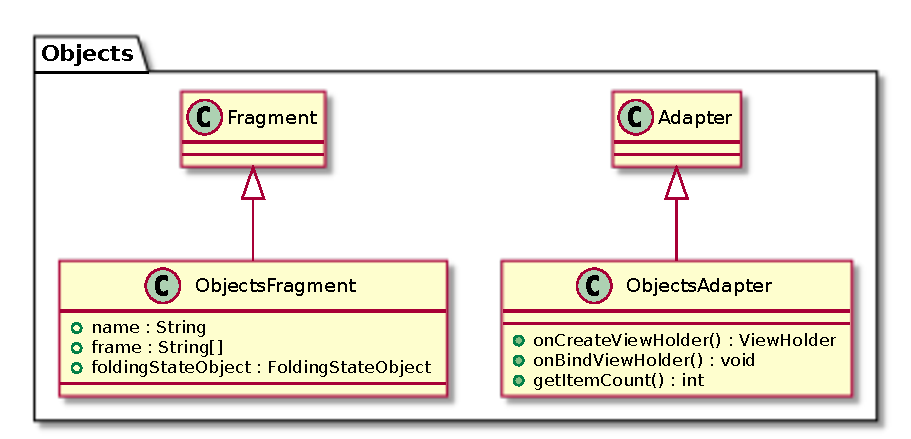
\includegraphics[width=0.70\linewidth]{../schemas/Conception_detaillee/classe_objects.pdf}
    \captionof{figure}{Diagramme du package Objects}
\end{minipage}

\subparagraph{Philosophie de conception \newline} 

\medspace

Le package Objects possède la classe ObjectAdapter du RecyclerView qui permet d'afficher la liste des objets. Elle permet de faire le lien entre les fragments et le RecyclerView. 
Chaque objet est matérialisé dans la liste des objets par une instance de la classe ObjectsFragment. 

\subparagraph{Description structurelle \newline}

\medspace

\textbf{Attributs :}

N.A.

\textbf{Services offerts :}

La classe ObjectAdapter contient les opérations suivantes : 

\begin{itemize}
    \item \textbf{onCreateViewHolder() : ViewHolder} --- Opération qui permet de créer un objet ViewHolder qui représente la vue d'un élément individuel dans le RecyclerView. 
    \item \textbf{onBindViewHolder() : void} --- Opération qui permet de lier les données d'un objet à la vue correspondante dans le RecyclerView. Elle est appelée lorsque le RecyclerView souhaite afficher ou mettre à jour les données d'un élément spécifique. 
    \item \textbf{getItemCount() : int} --- Opération qui permet de renvoyer le nombre total d'éléments dans la liste de données de l'adaptateur. Elle est utilisée par le RecyclerView pour déterminer combien d'éléments doivent être affichés.
\end{itemize}

\paragraph{La classe ObjectFragment}

\begin{minipage}
    {\linewidth}
    \centering
    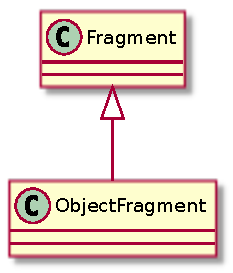
\includegraphics[width=0.40\linewidth]{../schemas/Conception_detaillee/classe_objectFragment.pdf}
    \captionof{figure}{Diagramme de classe de ObjectFragment}
\end{minipage}

\subparagraph{Philosophie de conception \newline} 

\medspace

La classe ObjectFragment est la classe associée à chaque fragment d'objet. Cette classe a pour rôle de créer un objet sur l'IHM et de lui associer ses trames.
Dans cette classe on détecte aussi si Utilisateur souhaite ajouter de nouvelles trames. 


\subparagraph{Description structurelle \newline}

\medspace

\textbf{Attributs :}

Les attribut associés à chaque objets sont : 
\begin{itemize}
    \item String name --- nom de l'objet
    \item String[] frame --- trames associées
    \item FoldingStateObject foldingStateObject --- état de l'objet (replié ou déplié)
\end{itemize}

\textbf{Services offerts :}

N.A.

\paragraph{L'énumération FoldingStateObject}

\begin{minipage}
    {\linewidth}
    \centering
    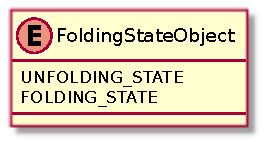
\includegraphics[width=0.40\linewidth]{../schemas/Conception_detaillee/classe_foldingStateObject.pdf}
    \captionof{figure}{Diagramme de l'énumération FoldingStateObject}
\end{minipage}

\subparagraph{Philosophie de conception \newline} 

\medspace

L'énumération FoldingStateObject permet de répertorier les deux états dans lesquels un objet peut être affiché. L'objet est visible sur l'écran, soit sous forme déplié (on peut observer les trames qu'il possède) soit sous forme replié (les potentielles trames qu'il possède ne sont pas visibles). Chaque objet visible sur l'écran possède cet attribut.

\subparagraph{Description structurelle \newline}

\medspace

\textbf{Attributs :}

N.A.

\textbf{Services offerts :}

\begin{itemize}
    \item \textbf{UNFOLDING\_STATE} --- Correspond à l'état déplié de l'objet (on observe les trames qu'il possède).
    \item \textbf{FOLDING\_STATE} --- Correspond à l'état replié de l'objet (les trames ne sont pas visibles).
\end{itemize}






% Diagramme de classe de MainActivityViewModel
\paragraph{La classe MainActivityViewModel}

\begin{minipage}
    {\linewidth}
    \centering
    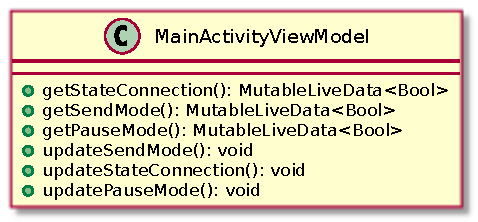
\includegraphics[width=0.80\linewidth]{../schemas/Conception_detaillee/classe_mainActivityViewModel.pdf}
    \captionof{figure}{Diagramme de classe de MainActivityViewModel}
\end{minipage}

\subparagraph{Philosophie de conception \newline} 

\medspace

La classe MainActivityViewModel a pour rôle de de mettre à jour l'affichage des boutons en fonctions des différents états de l'application. 

\subparagraph{Description structurelle \newline}

\medspace

\textbf{Attributs :}

N.A. 

\textbf{Services offerts :}

\begin{itemize}
    \item \textbf{getStateConnection(): MutableLiveData<Bool>} --- Opération qui retourne l'état de la connexion. 
    \item \textbf{getSendMode(): MutableLiveData<Bool>} --- Opération qui retourne l'état du mode d'envoi.
    \item \textbf{getPauseMode(): MutableLiveData<Bool>} --- Opération qui retourne l'état du mode pause ou play du sniffer.
    \item \textbf{updateSendMode(): void } --- Opération qui défini la valeur du mode d'envoi. 
    \item \textbf{updateStateConnection(): void} --- Opération qui défini la valeur de la connexion. 
    \item \textbf{updatePauseMode(): void} --- Opération qui défini la valeur du mode pause ou play du sniffer.
\end{itemize}

\subsubsection{Description des classes de CANgateway}

\paragraph{Diagramme de classes de CANgateway}

\begin{minipage}
    {\linewidth}
    \centering
    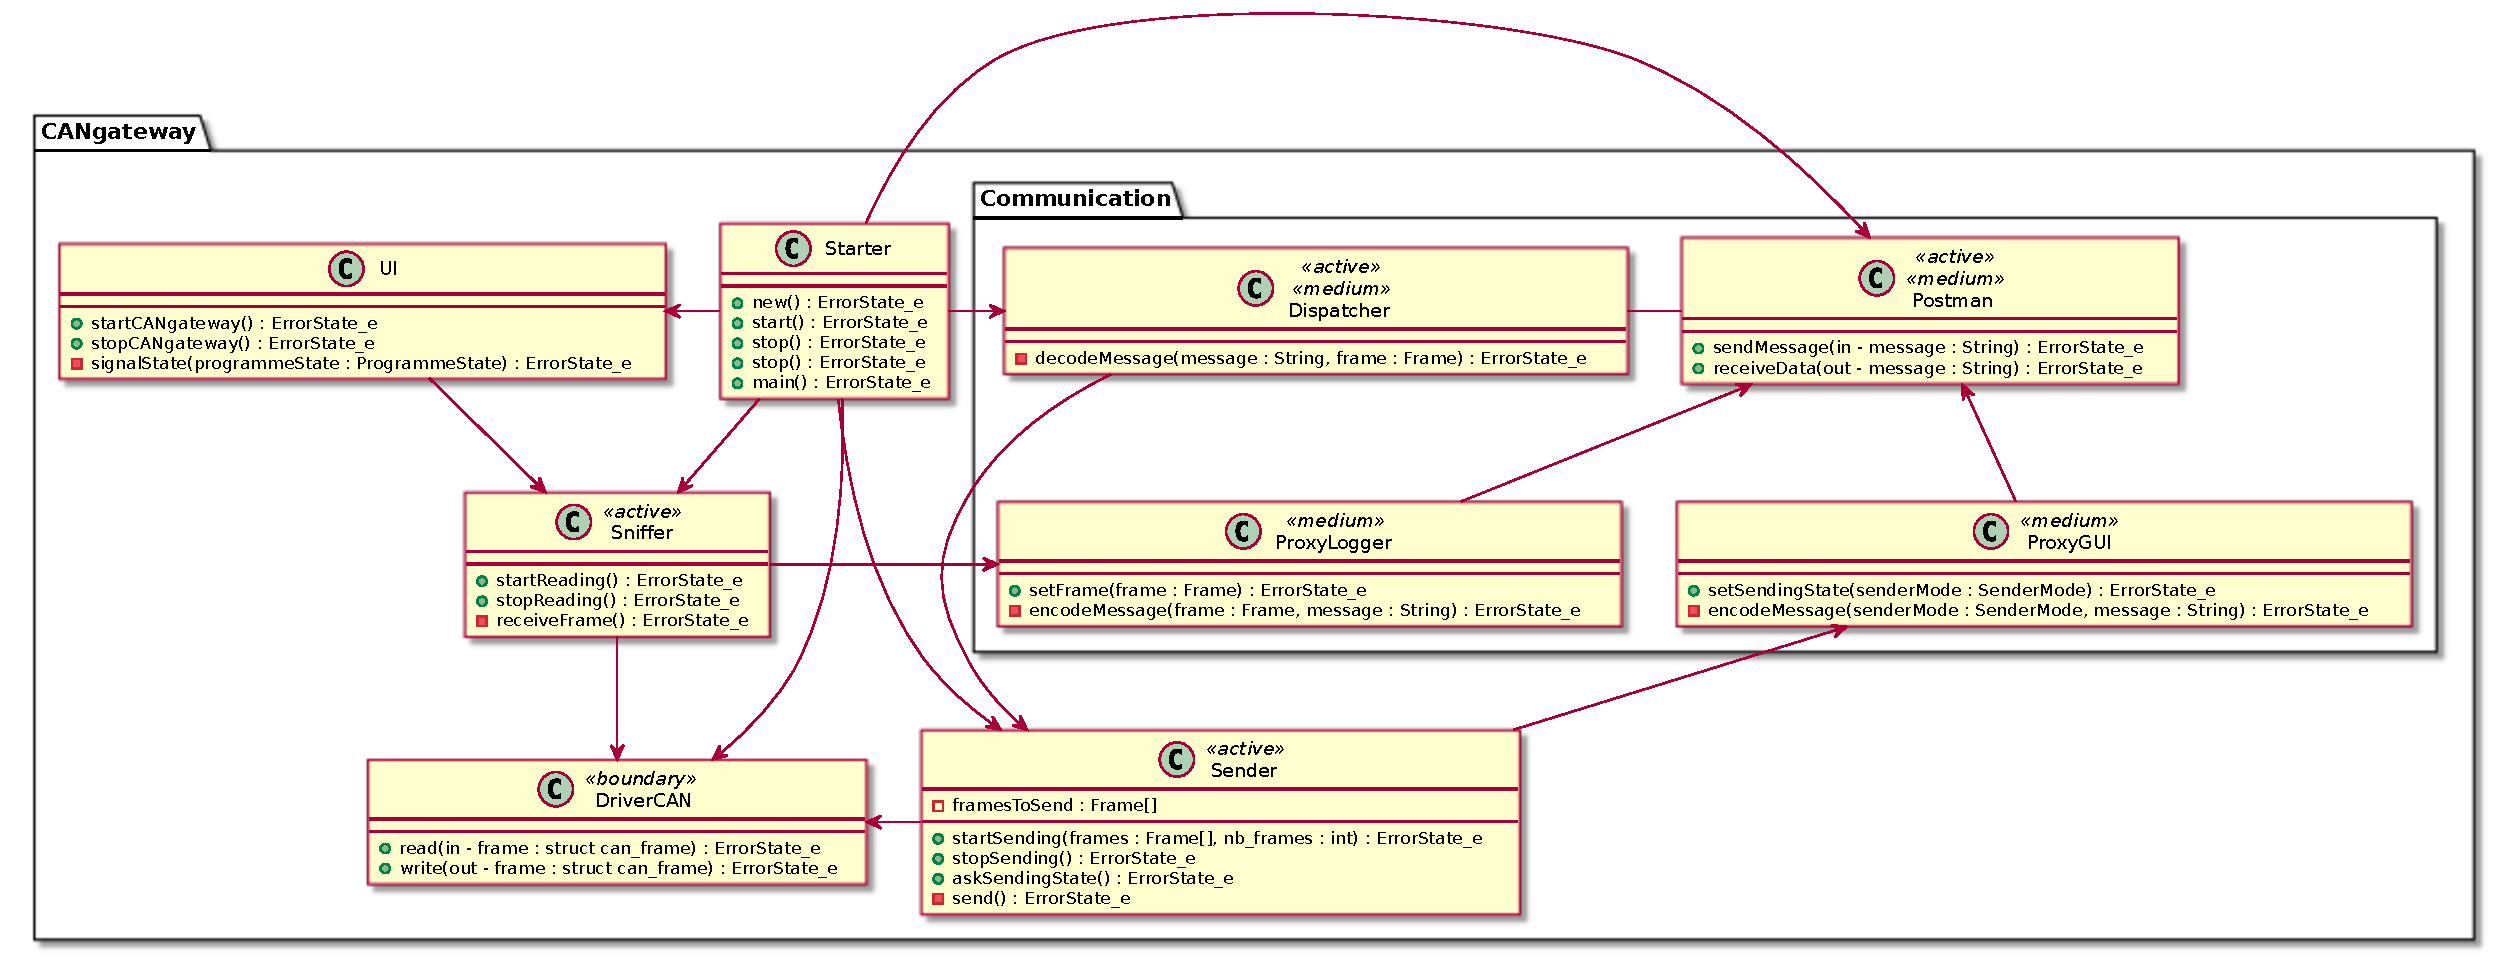
\includegraphics[width=\linewidth]{../schemas/Conception_detaillee/diag_classe_CANgateway.pdf}
    \captionof{figure}{Diagramme de classes de CANgateway}
\end{minipage}

\medspace

Le diagramme de classes de la figure ci-dessus représente l'architecture du programme {\nomLogiciel}. Cette architecture ne respecte pas totalement l'architecture de la conception générale due à l'implémentation d'une gestion d'erreur en C qui change donc les types de retours des fonctions. 
Ces fonctions retournent un état d'erreur de la forme : 
\begin{itemize}
    \item Enumération ErrorState\_e
    \item \'Eléments : 
    \item \begin{itemize}
        \item ERROR\_STATE\_SUCCESS : si tout se passe bien 
        \item ERROR\_STATE\_FAILURE : s'il y a au moins une erreur
        \item ERROR\_STATE\_TIMEOUT : si la cause de l'erreur est un timeout
    \end{itemize}
\end{itemize} 

\paragraph{La classe Starter}

\begin{minipage}
    {\linewidth}
    \centering
    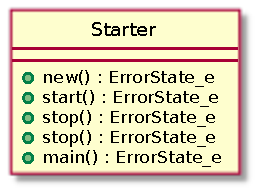
\includegraphics[width=0.30\linewidth]{../schemas/Conception_detaillee/classe_starter.pdf}
    \captionof{figure}{Diagramme de classe de Starter}
\end{minipage}

\subparagraph{Philosophie de conception \newline} 

\medspace

La classe Starter a pour rôle de créer et d'initialiser les classes qui seront utilisées par le programme {\nomLogiciel}.

Les objets créés sont les suivants :
\begin{itemize}
    \item UI,
    \item Sender
    \item Sniffer
    \item DriverCAN
    \item Postman
    \item Dispatcher
\end{itemize}

\subparagraph{Description structurelle \newline}

\medspace

\textbf{Attributs :}

N.A.

\textbf{Services offerts :}

\begin{itemize}
    \item \textbf{new() : ErrorState\_e} --- Opération qui crée les objets \textit{ui}, \textit{sender}, \textit{sniffer}, \textit{driverCAN}, \textit{dispatcher} et \textit{postman}.
    \item \textbf{start() : ErrorState\_e} --- Opération qui lance le programme {\nomLogiciel}.
    \item \textbf{stop() : ErrorState\_e} --- Opération qui arrête le programme {\nomLogiciel}.
    \item \textbf{free() : ErrorState\_e} --- Opération qui libère la mémoire allouée à l'objet Starter et à tous les objets qu'il a créés.
    \item \textbf{main() : int} --- Point d'entrée du programme. Opération qui instancie tous les objets et lance le programme {\nomLogiciel}.
\end{itemize}


\newpage 

\subparagraph{Séquence de démarrage et arrêt de {\nomLogiciel} \newline}

\medspace

\begin{minipage}
    {\linewidth}
    \centering
    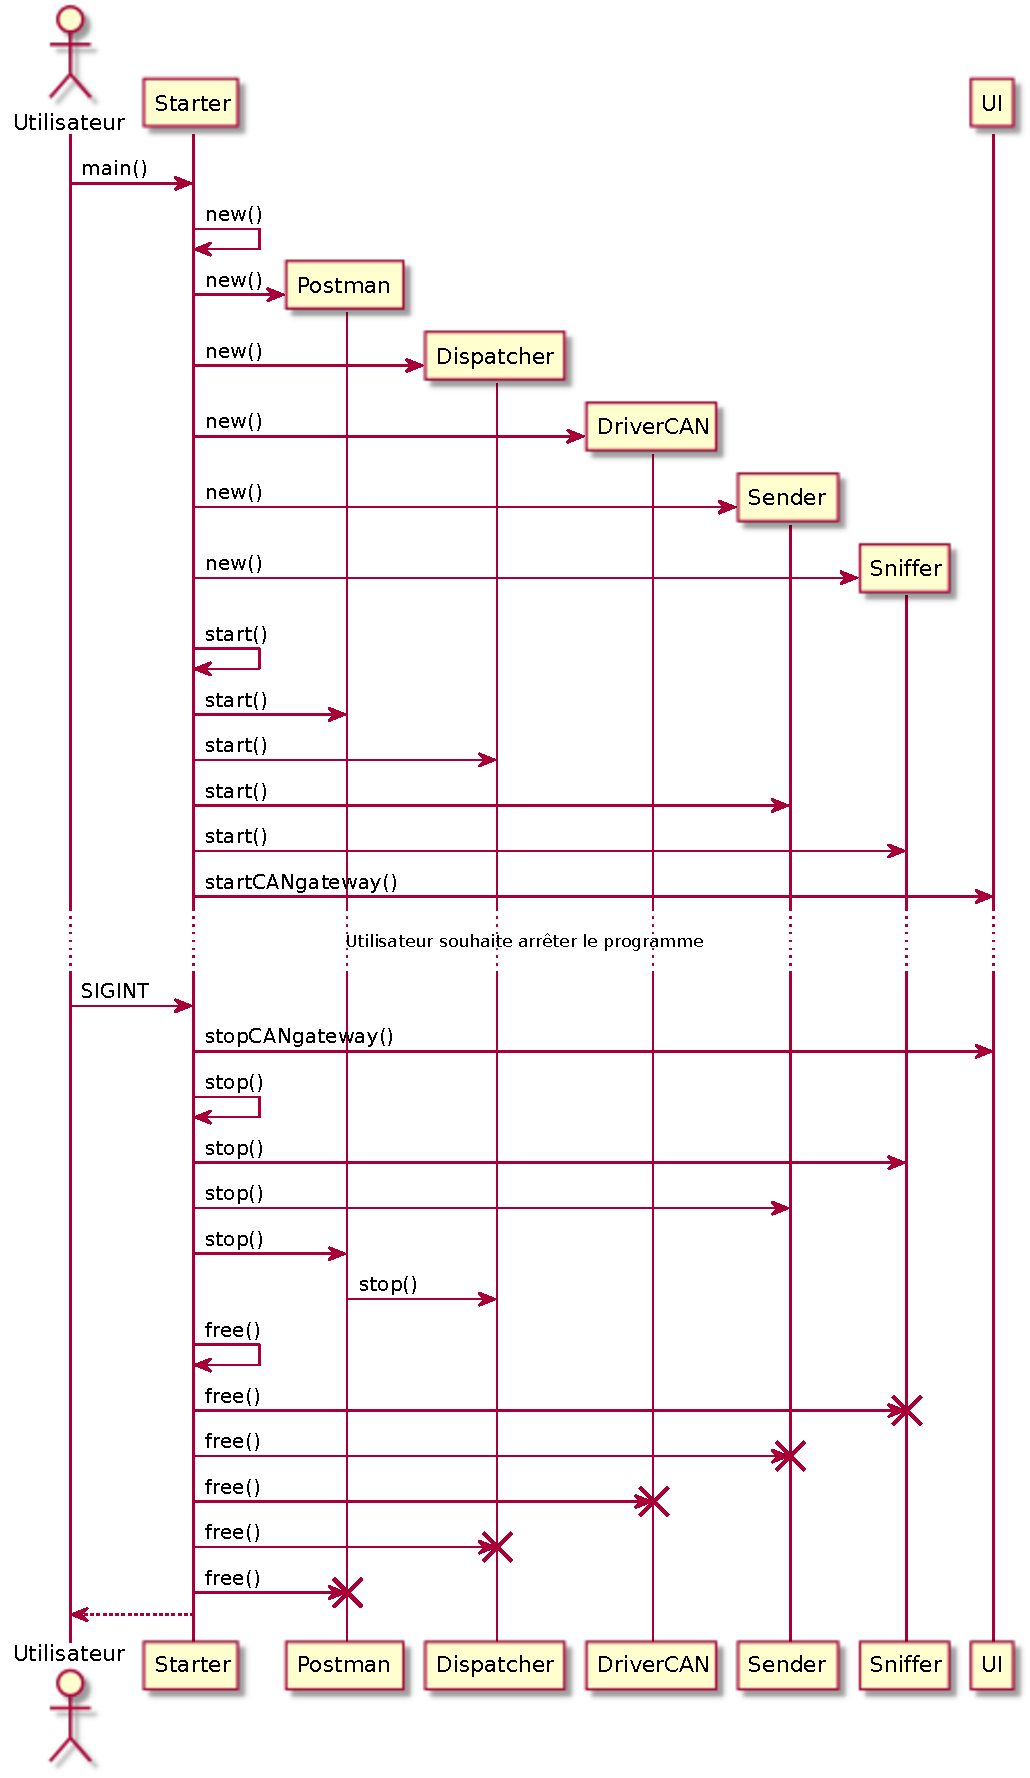
\includegraphics[height=0.9\textheight]{../schemas/Conception_detaillee/diag_sequence_Starter.pdf}
    \captionof{figure}{Diagramme de séquence de démarrage de {\nomLogiciel}}
\end{minipage}


\paragraph{La classe DriverCAN}

\begin{minipage}
    {\linewidth}
    \centering
    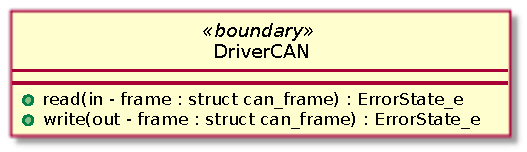
\includegraphics[width=0.50\linewidth]{../schemas/Conception_detaillee/classe_driverCAN.pdf}
    \captionof{figure}{Diagramme de classe de DriverCAN}
\end{minipage}

\subparagraph{Philosophie de conception \newline}

\medspace

La classe DriverCAN a pour rôle de communiquer avec le bus CAN. Elle est utilisée respectivement par les classes Sender et Sniffer pour envoyer et recevoir des trames sur le bus CAN. Cette classe utilise les SocketCAN pour communiquer avec le bus CAN et est donc dépendante de la bibliothèque can.h de Linux. 

\subparagraph{Description structurelle \newline}

\medspace

\textbf{Attributs :}
N.A.

\textbf{Services offerts :}

\begin{itemize}
    \item \textbf{write(in - frame : struct can\_frame) : ErrorState\_e} --- Opération qui envoie une trame sur le bus CAN. Elle renvoie un code d'erreur si l'envoi de la trame a réussi ou échoué.
    \item \textbf{read(out - frame : struct can\_frame) : ErrorState\_e} --- Opération qui lit une trame sur le bus CAN. Elle renvoie un code d'erreur si la lecture de la trame a réussi ou échoué.
\end{itemize}

\paragraph{La classe Dispatcher}


\begin{minipage}
    {\linewidth}
    \centering
    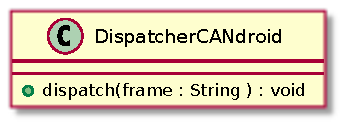
\includegraphics[width=0.50\linewidth]{../schemas/Conception_detaillee/classe_dispatcher_candroid.pdf}
    \captionof{figure}{Diagramme de classe de DispatcherCANdroid}
\end{minipage}
\subparagraph{Philosophie de conception \newline} 

\medspace


La classe DispatcherCANdroid a pour objectif de faciliter la communication. Elle joue le rôle d'intermédiaire entre la classe CommunicationCANdroid et la classe LogManager. Elle permet une communication centralisée et efficace dans l'application {\nomApplication}. 

\subparagraph{Description structurelle \newline}


\medspace

\textbf{Attributs :}

N.A.

\textbf{Services offerts :}

\begin{itemize}
    \item \textbf{dispatch(frame : String) : void} --- Opération qui permet l'envoi de la trame vers logManager pour ensuite l'afficher. 
\end{itemize}

\paragraph{La classe Postman}

\begin{minipage}
    {\linewidth}
    \centering
    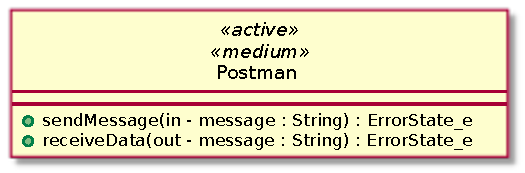
\includegraphics[width=0.50\linewidth]{../schemas/Conception_detaillee/classe_postman.pdf}
    \captionof{figure}{Diagramme de classe de Postman}
\end{minipage}

\subparagraph{Philosophie de conception \newline} 

\medspace

Postman est une classe qui permet de communiquer avec l'application {\nomApplication}. Elle échange divers messages avec l'application suivant le protocole de communication défini dans la \autoref{protocole_com}.

\subparagraph{Description structurelle \newline}

\medspace

\textbf{Attributs :}

N.A.

\textbf{Services offerts :}

\begin{itemize}
    \item \textbf{sendMessage(in - message : String) : ErrorState\_e} --- Opération qui permet d'envoyer un message à l'application {\nomApplication}.
    \item \textbf{receiveData(out - message : String) : ErrorState\_e} --- Opération qui permet de recevoir un message de l'application {\nomApplication}.
\end{itemize}


\paragraph{La classe ProxyGUI}

\begin{minipage}
    {\linewidth}
    \centering
    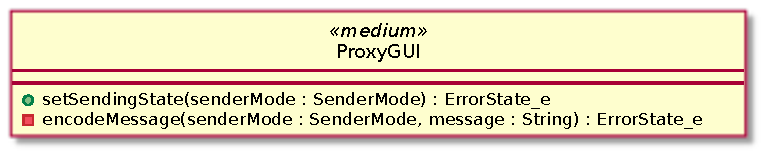
\includegraphics[width=0.65\linewidth]{../schemas/Conception_detaillee/classe_proxyGUI.pdf}
    \captionof{figure}{Diagramme de classe de ProxyGUI}
\end{minipage}

\subparagraph{Philosophie de conception \newline} 

\medspace

La classe ProxyGUI qui est dans le programme {\nomLogiciel} a pour rôle de simuler le comportement de la classe GUI présente dans l'application {\nomApplication}. Toutes les requêtes que Sender doit envoyer à GUI passent par cette classe.

\subparagraph{Description structurelle \newline}

\medspace

\textbf{Attributs :}

N.A.

\textbf{Services offerts :}

\begin{itemize}
    \item \textbf{setSendingState(senderMode : SenderMode) : ErrorState\_e} --- Opération qui permet de définir l'état du Mode Envoi du système.
    \item \textbf{encodeMessage(senderMode : SenderMode, message : String) : ErrorState\_e} --- Opération qui permet d'encoder un état du Mode Envoi en une chaine de caractère.
\end{itemize}


\paragraph{La classe ProxyLogger}

\begin{minipage}
    {\linewidth}
    \centering
    \includegraphics[width=0.65\linewidth]{../schemas/Conception_detaillee/classe_ProxyLogger.pdf}
    \captionof{figure}{Diagramme de classe de ProxyLogger}
\end{minipage}

\subparagraph{Philosophie de conception \newline} 

\medspace

La classe ProxyLogger qui est dans le programme {\nomLogiciel} a pour rôle de simuler le comportement de la classe Logger présente dans l'application {\nomApplication}.

\subparagraph{Description structurelle \newline}

\medspace

\textbf{Attributs :}

N.A.

\textbf{Services offerts :}

\begin{itemize}
    \item \textbf{setFrame(frame : Frame) : ErrorState\_e} --- Opération qui permet de fournir les trames sniffées au Logger.
    \item \textbf{encodeMessage(frame : Frame, message : String) : ErrorState\_e} --- Opération qui permet d'encoder une trame en une chaîne de caractères.
\end{itemize}


\newpage 

% Protocole de communication
\subsection{Protocole de communication} \label{protocole_com}

Notre protocole de communication repose sur l'utilisation de sockets TCP/IP. Les données échangées sont des chaînes de caractères, assurant ainsi un protocole textuel.

\subsubsection{Protocole de communication de {\nomApplication} vers {\nomLogiciel}}

\paragraph{Formalisation du protocole}
\label{sec:formalisation-protocole-CANdroidToCANgateway}

Lors de la schématisation des formats des messages, nous avons choisi de séparer les parties des messages par des espaces pour des questions de lisibilité. Cependant, ces espaces ne sont pas présents lors de l'exécution du protocole. Par conséquent, nous ne les avons pas représentés dans la partie \ref{sec:exemple-CANdroidToCANgateway}.\\

L'application {\nomApplication} transmet trois types d'informations au programme {\nomLogiciel} : une demande de l'état du Mode Envoi, une demande d'arrêt d'envoi des trames et une séquence de trames.\\

Lorsque Utilisateur envoie des trames, l'application {\nomApplication} transmet un message lui-même composé de plusieurs messages correspondant à des chaînes de caractères. Ce message comprend : un message indiquant le nombre trames envoyées dans la séquence, et un message par trame de la séquence. L'application {\nomApplication} envoie donc une donnée sous le format suivant :\\

\begin{minipage}
    \textwidth
    \centering
    \begin{tabular}{|c|c|c|}
        \hline
        nb= N \textbackslash n & \# ID \$ LENGTH @ DATA / PERIODICITY \textbackslash n & ...\\
        \hline
    \end{tabular}
\end{minipage}

\medspace

\begin{itemize}
    \item \textbf{nb=} : indique que la suite du message sera N ;
    \item \textbf{N} : correspond au nombre de trames dans la séquence à envoyer ;
    \item \textbf{\textbackslash n} : caractère de fin du message, indiquant que le prochain message sera la première trame de la séquence ;
    \item \textbf{\#} : indique que la suite du message est ID ;
    \item \textbf{ID} : ID de la trame CAN lu sur le réseau CAN. ID correspond à un nombre hexadécimal à 3 chiffre. Dans notre cas, nous traitons des trames au format standard, ID peut donc prendre une valeur minimale de 0x000 et une valeur maximale de 0x7FF, ce qui correspond à 2047 en décimal ;
    \item \textbf{\$} : séparateur entre ID et LENGTH ;
    \item \textbf{LENGTH} : taille de la trame. Cette valeur est un entier qui correspond à un nombre d'octet. Au format standard, une trame a une longueur maximale de 8 octets, LENGTH va donc de 0 à 8 ;
    \item \textbf{@} : séparateur entre LENGTH et DATA ;
    \item \textbf{DATA} : correspond aux données de la trame. Au format standard, on peut avoir jusqu'à 8 octets de données, où chaque octet peut contenir une valeur hexadécimale allant de 0x00 à 0xFF ;
    \item \textbf{/} : séparateur entre DATA et PERIODICITY ;
    \item \textbf{PERIODICITY} : correspond à la périodicité de l'envoi de la trame. Cette valeur est un entier qui a pour valeur minimale 0, et n'a pas de valeur maximale. Cette valeur est en milliseconde ;
    \item \textbf{\textbackslash n} : caractère de fin de message ;
    \item \textbf{...} : représente les N autres trames de la séquence.\\
\end{itemize}

Utilisateur peut demander l'arrêt d'envoi des trames. L'application {\nomApplication} envoie alors une demande d'état du Mode Envoi sous forme de chaîne de caractères. Cette donnée est envoyée sous le format suivant : \\

\begin{minipage}
    \textwidth
    \centering
    \begin{tabular}{|c|}
        \hline
        ! \textbackslash n\\
        \hline
    \end{tabular}
\end{minipage}

\medspace

\begin{itemize}
    \item \textbf{!} : caractère définissant la nature du message, c'est-à-dire une demande d'arrêt du Mode Envoi ;
    \item \textbf{\textbackslash n} : caractère de fin de message.\\
\end{itemize}


Lorsque Utilisateur souhaite envoyer des trames, ou arrêter l'envoi de trames, le Mode Envoi doit être mis à jour. L'application {\nomApplication} envoie alors une demande d'état du Mode Envoi sous forme de chaîne de caractères. Cette donnée est envoyée sous le format suivant :\\

\begin{minipage}
    \textwidth
    \centering
    \begin{tabular}{|c|}
        \hline
        ? \textbackslash n\\
        \hline
    \end{tabular}
\end{minipage}

\medspace

\begin{itemize}
    \item \textbf{?} : caractère définissant la nature du message, c'est-à-dire une demande d'état du Mode Envoi ;
    \item \textbf{\textbackslash n} : caractère de fin de message.\\
\end{itemize}

\paragraph{Exemples}
\label{sec:exemple-CANgatewayToCANdroid}

Pour rappel, nous appliquons un protocole textuel, les données envoyées sont sous la forme de chaîne de caractères.


\subparagraph{Recevoir des trames \newline}

\medspace

Les échanges présentés dans le diagramme de la \autoref{fig:inter-CU_Recevoir_des_trames_-_Scénario_nominal} représente un envoi de donnée du programme {\nomLogiciel} vers l'application {\nomApplication} via le protocole de communication décrit dans le \autoref{sec:formalisation-protocole-CANgatewayToCANdroid}. Cette donnée correspond à une trame et peut être de la forme suivante :\\

\begin{minipage}
    \textwidth
    \centering
    \begin{tabular}{|c|}
        \hline
        \textasciitilde{}frame\#19B\$6@00000E000000\textbackslash n\\
        \hline
    \end{tabular}
\end{minipage}

\medspace

Cette trame permet d'ouvrir la porte avant-gauche de la portière sur le Simulateur ICSim.


\subparagraph{Envoyer des trames \newline}

\medspace

Les échanges présentés dans le diagramme de la \autoref{fig:inter-CU_Envoyer_des_trames_-_Scénario_nominal} représente un envoi de donnée du programme {\nomLogiciel} vers l'application {\nomApplication} via le protocole de communication décrit dans le \autoref{sec:formalisation-protocole-CANgatewayToCANdroid}. Il y a deux données transmises lors d'un envoi de trames :
\begin{itemize}
    \item L'état du Mode Envoi ;
    \item La trame envoyée.
\end{itemize} 
L'état du Mode Envoi est de la forme suivante :\\

\begin{minipage}
    \textwidth
    \centering
    \begin{tabular}{|c|}
        \hline
        \textasciitilde{}sendingState\#1\textbackslash n\\
        \hline
    \end{tabular}
\end{minipage}

\medspace

La trame envoyée est de la forme suivante :\\

\begin{minipage}
    \textwidth
    \centering
    \begin{tabular}{|c|}
        \hline
        \textasciitilde{}frame\#19B\$6@00000E000000\textbackslash n\\
        \hline
    \end{tabular}
\end{minipage}

\medspace

\subparagraph{Arrêter d'envoyer des trames \newline}

\medspace

Les échanges présentés dans le diagramme de la \autoref{fig:inter-CU_Arrêter_envoi_des_trames_-_Scénario_nominal} représente un envoi de donnée du programme {\nomLogiciel} vers l'application {\nomApplication} via le protole de communication décrit dans le \autoref{sec:formalisation-protocole-CANgatewayToCANdroid}. Cette donnée correspond à un état du Mode Envoi et est de la forme suivante :\\

\begin{minipage}
    \textwidth
    \centering
    \begin{tabular}{|c|}
        \hline
        \textasciitilde{}sendingState\#0\textbackslash n\\
        \hline
    \end{tabular}
\end{minipage}

\subsubsection{Protocole de communication de {\nomLogiciel} vers {\nomApplication}}

\paragraph{Formalisation du protocole}
\label{sec:formalisation-protocole-CANdroidToCANgateway}

Lors de la schématisation des formats des messages, nous avons choisi de séparer les parties des messages par des espaces pour des questions de lisibilité. Cependant, ces espaces ne sont pas présents lors de l'exécution du protocole. Par conséquent, nous ne les avons pas représentés dans la partie \ref{sec:exemple-CANdroidToCANgateway}.\\

L'application {\nomApplication} transmet trois types d'informations au programme {\nomLogiciel} : une demande de l'état du Mode Envoi, une demande d'arrêt d'envoi des trames et une séquence de trames.\\

Lorsque Utilisateur envoie des trames, l'application {\nomApplication} transmet un message lui-même composé de plusieurs messages correspondant à des chaînes de caractères. Ce message comprend : un message indiquant le nombre trames envoyées dans la séquence, et un message par trame de la séquence. L'application {\nomApplication} envoie donc une donnée sous le format suivant :\\

\begin{minipage}
    \textwidth
    \centering
    \begin{tabular}{|c|c|c|}
        \hline
        nb= N \textbackslash n & \# ID \$ LENGTH @ DATA / PERIODICITY \textbackslash n & ...\\
        \hline
    \end{tabular}
\end{minipage}

\medspace

\begin{itemize}
    \item \textbf{nb=} : indique que la suite du message sera N ;
    \item \textbf{N} : correspond au nombre de trames dans la séquence à envoyer ;
    \item \textbf{\textbackslash n} : caractère de fin du message, indiquant que le prochain message sera la première trame de la séquence ;
    \item \textbf{\#} : indique que la suite du message est ID ;
    \item \textbf{ID} : ID de la trame CAN lu sur le réseau CAN. ID correspond à un nombre hexadécimal à 3 chiffre. Dans notre cas, nous traitons des trames au format standard, ID peut donc prendre une valeur minimale de 0x000 et une valeur maximale de 0x7FF, ce qui correspond à 2047 en décimal ;
    \item \textbf{\$} : séparateur entre ID et LENGTH ;
    \item \textbf{LENGTH} : taille de la trame. Cette valeur est un entier qui correspond à un nombre d'octet. Au format standard, une trame a une longueur maximale de 8 octets, LENGTH va donc de 0 à 8 ;
    \item \textbf{@} : séparateur entre LENGTH et DATA ;
    \item \textbf{DATA} : correspond aux données de la trame. Au format standard, on peut avoir jusqu'à 8 octets de données, où chaque octet peut contenir une valeur hexadécimale allant de 0x00 à 0xFF ;
    \item \textbf{/} : séparateur entre DATA et PERIODICITY ;
    \item \textbf{PERIODICITY} : correspond à la périodicité de l'envoi de la trame. Cette valeur est un entier qui a pour valeur minimale 0, et n'a pas de valeur maximale. Cette valeur est en milliseconde ;
    \item \textbf{\textbackslash n} : caractère de fin de message ;
    \item \textbf{...} : représente les N autres trames de la séquence.\\
\end{itemize}

Utilisateur peut demander l'arrêt d'envoi des trames. L'application {\nomApplication} envoie alors une demande d'état du Mode Envoi sous forme de chaîne de caractères. Cette donnée est envoyée sous le format suivant : \\

\begin{minipage}
    \textwidth
    \centering
    \begin{tabular}{|c|}
        \hline
        ! \textbackslash n\\
        \hline
    \end{tabular}
\end{minipage}

\medspace

\begin{itemize}
    \item \textbf{!} : caractère définissant la nature du message, c'est-à-dire une demande d'arrêt du Mode Envoi ;
    \item \textbf{\textbackslash n} : caractère de fin de message.\\
\end{itemize}


Lorsque Utilisateur souhaite envoyer des trames, ou arrêter l'envoi de trames, le Mode Envoi doit être mis à jour. L'application {\nomApplication} envoie alors une demande d'état du Mode Envoi sous forme de chaîne de caractères. Cette donnée est envoyée sous le format suivant :\\

\begin{minipage}
    \textwidth
    \centering
    \begin{tabular}{|c|}
        \hline
        ? \textbackslash n\\
        \hline
    \end{tabular}
\end{minipage}

\medspace

\begin{itemize}
    \item \textbf{?} : caractère définissant la nature du message, c'est-à-dire une demande d'état du Mode Envoi ;
    \item \textbf{\textbackslash n} : caractère de fin de message.\\
\end{itemize}

\paragraph{Exemples}
\label{sec:exemple-CANgatewayToCANdroid}

Pour rappel, nous appliquons un protocole textuel, les données envoyées sont sous la forme de chaîne de caractères.


\subparagraph{Recevoir des trames \newline}

\medspace

Les échanges présentés dans le diagramme de la \autoref{fig:inter-CU_Recevoir_des_trames_-_Scénario_nominal} représente un envoi de donnée du programme {\nomLogiciel} vers l'application {\nomApplication} via le protocole de communication décrit dans le \autoref{sec:formalisation-protocole-CANgatewayToCANdroid}. Cette donnée correspond à une trame et peut être de la forme suivante :\\

\begin{minipage}
    \textwidth
    \centering
    \begin{tabular}{|c|}
        \hline
        \textasciitilde{}frame\#19B\$6@00000E000000\textbackslash n\\
        \hline
    \end{tabular}
\end{minipage}

\medspace

Cette trame permet d'ouvrir la porte avant-gauche de la portière sur le Simulateur ICSim.


\subparagraph{Envoyer des trames \newline}

\medspace

Les échanges présentés dans le diagramme de la \autoref{fig:inter-CU_Envoyer_des_trames_-_Scénario_nominal} représente un envoi de donnée du programme {\nomLogiciel} vers l'application {\nomApplication} via le protocole de communication décrit dans le \autoref{sec:formalisation-protocole-CANgatewayToCANdroid}. Il y a deux données transmises lors d'un envoi de trames :
\begin{itemize}
    \item L'état du Mode Envoi ;
    \item La trame envoyée.
\end{itemize} 
L'état du Mode Envoi est de la forme suivante :\\

\begin{minipage}
    \textwidth
    \centering
    \begin{tabular}{|c|}
        \hline
        \textasciitilde{}sendingState\#1\textbackslash n\\
        \hline
    \end{tabular}
\end{minipage}

\medspace

La trame envoyée est de la forme suivante :\\

\begin{minipage}
    \textwidth
    \centering
    \begin{tabular}{|c|}
        \hline
        \textasciitilde{}frame\#19B\$6@00000E000000\textbackslash n\\
        \hline
    \end{tabular}
\end{minipage}

\medspace

\subparagraph{Arrêter d'envoyer des trames \newline}

\medspace

Les échanges présentés dans le diagramme de la \autoref{fig:inter-CU_Arrêter_envoi_des_trames_-_Scénario_nominal} représente un envoi de donnée du programme {\nomLogiciel} vers l'application {\nomApplication} via le protole de communication décrit dans le \autoref{sec:formalisation-protocole-CANgatewayToCANdroid}. Cette donnée correspond à un état du Mode Envoi et est de la forme suivante :\\

\begin{minipage}
    \textwidth
    \centering
    \begin{tabular}{|c|}
        \hline
        \textasciitilde{}sendingState\#0\textbackslash n\\
        \hline
    \end{tabular}
\end{minipage}



\newpage 

% Gestion multitâche
\subsection{Gestion du multitâche}

\subsubsection{Identification des accès concurrents}

\paragraph{Côté CANdroid}

\medspace

\begin{minipage}
    \textwidth
    \centering
    \begin{tabular}{|c|c|c|c|}
        \hline
        Tâches & ConnectionCANdroid & ProtocolCANdroid & DispatcherCANdroid \\
        \hline
        GUI & & &\\
        \hline
        Interface DAO & & &\\
        \hline
        CommunicationCANdroid & X & X & X \\
        \hline
    \end{tabular}
    \captionof{table}{Accès concurrents côté CANdroid}
\end{minipage}

\medspace

\textbf{Analyse :} GUI est considéré ici en tant que package car il correspond à l'interface dans sa globalité. Il n'y a pas de potentiels accès concurrents car uniquement CommunicationCANdroid peut accéder aux opérations liées à la connexion. L'interface ne peut pas poser de potentiels accès concurrents car l'appel des opérations de l'interface se font via un ExecutorService, qui va s'assurer de ne pas bloquer le thread principal. De son coté, GUI va être utilisé par l'UI Thread et donc a son propre thread et ne peut pas poser de problèmes d'accès concurrents. 

\paragraph{Côté CANgateway}

\medspace

\begin{minipage}
    \textwidth
    \centering
    \begin{tabular}{|c|c|c|c|}
        \hline
        Tâches & DriverCAN & ProxyLogger & ProxyGUI\\
        \hline
        UI &  &  &\\
        \hline
        Postman &  &  & \\
        \hline
        Dispatcher &  &  & \\
        \hline
        Sniffer & X & X &  \\
        \hline
        Sender & X & X & X \\
        \hline
    \end{tabular}
    \captionof{table}{Accès concurrents côté CANgateway}
\end{minipage}

\medspace

\textbf{Analyse générale :} Il y a de potentiels accès concurrents entre les tâches Sniffer et Sender. En effet, ces deux tâches utilisent la classe DriverCAN pour communiquer avec le bus CAN et la classe ProxyLogger pour informer l'application {\nomApplication} des trames envoyées et reçues sur le bus CAN. Il est donc nécessaire de protéger les accès concurrents à ces classes.\\

\textbf{Problèmes avec la classe ProxyLogger :} En réalité, il n'y a pas de problèmes d'accès concurrents avec la classe ProxyLogger car elle utilise la classe Postman afin de transmettre les informations à fournir à Logger et que cette classe est déjà protégée contre les accès concurrents.\\

\textbf{Problèmes avec la classe DriverCAN :} La classe DriverCAN utilise les socketCAN pour communiquer avec le bus CAN. Or les classes Sender et Sniffer utilisent deux sockets différentes. La classe Sender n'utilise sa socketCAN que pour écrire sur le bus. À l'inverse, la classe Sniffer n'utilise sa socketCAN que pour lire sur le bus. Il n'y a donc pas de réels problèmes d'accès concurrents.\\ 



% Gestion persistance
\subsection{Gestion de la persistance}

\medskip

Afin de gérer la persistance des données dans l'application {\nomApplication}, une base de données a été utilisée. Cette base de données se décompose en deux classes qui sont les objets Object et les trames Frame. Ces deux classes consitituent le coeur de la base de données. 
Il y a également une interface appelée DAO, qui permet de faire des recherches dans la base de données. Ces recherches sont des requêtes SQL appliquées à la base de données. Afin d'utiliser la base de données, une instance de la base de données est nécessaire, c'est l'utilité de la classe BDD. Cette instance de la base de données permet d'accéder à l'interface ainsi qu'à toutes ses requêtes. 
